% Options for packages loaded elsewhere
\PassOptionsToPackage{unicode}{hyperref}
\PassOptionsToPackage{hyphens}{url}
\PassOptionsToPackage{dvipsnames,svgnames,x11names}{xcolor}
%
\documentclass[
  letterpaper,
  DIV=11,
  numbers=noendperiod]{scrreprt}

\usepackage{amsmath,amssymb}
\usepackage{iftex}
\ifPDFTeX
  \usepackage[T1]{fontenc}
  \usepackage[utf8]{inputenc}
  \usepackage{textcomp} % provide euro and other symbols
\else % if luatex or xetex
  \usepackage{unicode-math}
  \defaultfontfeatures{Scale=MatchLowercase}
  \defaultfontfeatures[\rmfamily]{Ligatures=TeX,Scale=1}
\fi
\usepackage{lmodern}
\ifPDFTeX\else  
    % xetex/luatex font selection
\fi
% Use upquote if available, for straight quotes in verbatim environments
\IfFileExists{upquote.sty}{\usepackage{upquote}}{}
\IfFileExists{microtype.sty}{% use microtype if available
  \usepackage[]{microtype}
  \UseMicrotypeSet[protrusion]{basicmath} % disable protrusion for tt fonts
}{}
\makeatletter
\@ifundefined{KOMAClassName}{% if non-KOMA class
  \IfFileExists{parskip.sty}{%
    \usepackage{parskip}
  }{% else
    \setlength{\parindent}{0pt}
    \setlength{\parskip}{6pt plus 2pt minus 1pt}}
}{% if KOMA class
  \KOMAoptions{parskip=half}}
\makeatother
\usepackage{xcolor}
\setlength{\emergencystretch}{3em} % prevent overfull lines
\setcounter{secnumdepth}{5}
% Make \paragraph and \subparagraph free-standing
\ifx\paragraph\undefined\else
  \let\oldparagraph\paragraph
  \renewcommand{\paragraph}[1]{\oldparagraph{#1}\mbox{}}
\fi
\ifx\subparagraph\undefined\else
  \let\oldsubparagraph\subparagraph
  \renewcommand{\subparagraph}[1]{\oldsubparagraph{#1}\mbox{}}
\fi


\providecommand{\tightlist}{%
  \setlength{\itemsep}{0pt}\setlength{\parskip}{0pt}}\usepackage{longtable,booktabs,array}
\usepackage{calc} % for calculating minipage widths
% Correct order of tables after \paragraph or \subparagraph
\usepackage{etoolbox}
\makeatletter
\patchcmd\longtable{\par}{\if@noskipsec\mbox{}\fi\par}{}{}
\makeatother
% Allow footnotes in longtable head/foot
\IfFileExists{footnotehyper.sty}{\usepackage{footnotehyper}}{\usepackage{footnote}}
\makesavenoteenv{longtable}
\usepackage{graphicx}
\makeatletter
\def\maxwidth{\ifdim\Gin@nat@width>\linewidth\linewidth\else\Gin@nat@width\fi}
\def\maxheight{\ifdim\Gin@nat@height>\textheight\textheight\else\Gin@nat@height\fi}
\makeatother
% Scale images if necessary, so that they will not overflow the page
% margins by default, and it is still possible to overwrite the defaults
% using explicit options in \includegraphics[width, height, ...]{}
\setkeys{Gin}{width=\maxwidth,height=\maxheight,keepaspectratio}
% Set default figure placement to htbp
\makeatletter
\def\fps@figure{htbp}
\makeatother
\newlength{\cslhangindent}
\setlength{\cslhangindent}{1.5em}
\newlength{\csllabelwidth}
\setlength{\csllabelwidth}{3em}
\newlength{\cslentryspacingunit} % times entry-spacing
\setlength{\cslentryspacingunit}{\parskip}
\newenvironment{CSLReferences}[2] % #1 hanging-ident, #2 entry spacing
 {% don't indent paragraphs
  \setlength{\parindent}{0pt}
  % turn on hanging indent if param 1 is 1
  \ifodd #1
  \let\oldpar\par
  \def\par{\hangindent=\cslhangindent\oldpar}
  \fi
  % set entry spacing
  \setlength{\parskip}{#2\cslentryspacingunit}
 }%
 {}
\usepackage{calc}
\newcommand{\CSLBlock}[1]{#1\hfill\break}
\newcommand{\CSLLeftMargin}[1]{\parbox[t]{\csllabelwidth}{#1}}
\newcommand{\CSLRightInline}[1]{\parbox[t]{\linewidth - \csllabelwidth}{#1}\break}
\newcommand{\CSLIndent}[1]{\hspace{\cslhangindent}#1}

\usepackage{booktabs}
\usepackage{caption}
\usepackage{longtable}
\usepackage{colortbl}
\usepackage{array}
\KOMAoption{captions}{tableheading}
\makeatletter
\makeatother
\makeatletter
\@ifpackageloaded{bookmark}{}{\usepackage{bookmark}}
\makeatother
\makeatletter
\@ifpackageloaded{caption}{}{\usepackage{caption}}
\AtBeginDocument{%
\ifdefined\contentsname
  \renewcommand*\contentsname{Table of contents}
\else
  \newcommand\contentsname{Table of contents}
\fi
\ifdefined\listfigurename
  \renewcommand*\listfigurename{List of Figures}
\else
  \newcommand\listfigurename{List of Figures}
\fi
\ifdefined\listtablename
  \renewcommand*\listtablename{List of Tables}
\else
  \newcommand\listtablename{List of Tables}
\fi
\ifdefined\figurename
  \renewcommand*\figurename{Figure}
\else
  \newcommand\figurename{Figure}
\fi
\ifdefined\tablename
  \renewcommand*\tablename{Table}
\else
  \newcommand\tablename{Table}
\fi
}
\@ifpackageloaded{float}{}{\usepackage{float}}
\floatstyle{ruled}
\@ifundefined{c@chapter}{\newfloat{codelisting}{h}{lop}}{\newfloat{codelisting}{h}{lop}[chapter]}
\floatname{codelisting}{Listing}
\newcommand*\listoflistings{\listof{codelisting}{List of Listings}}
\makeatother
\makeatletter
\@ifpackageloaded{caption}{}{\usepackage{caption}}
\@ifpackageloaded{subcaption}{}{\usepackage{subcaption}}
\makeatother
\makeatletter
\@ifpackageloaded{tcolorbox}{}{\usepackage[skins,breakable]{tcolorbox}}
\makeatother
\makeatletter
\@ifundefined{shadecolor}{\definecolor{shadecolor}{rgb}{.97, .97, .97}}
\makeatother
\makeatletter
\makeatother
\makeatletter
\makeatother
\ifLuaTeX
  \usepackage{selnolig}  % disable illegal ligatures
\fi
\IfFileExists{bookmark.sty}{\usepackage{bookmark}}{\usepackage{hyperref}}
\IfFileExists{xurl.sty}{\usepackage{xurl}}{} % add URL line breaks if available
\urlstyle{same} % disable monospaced font for URLs
\hypersetup{
  pdftitle={IDR 4000 MAPPEEKSAMEN},
  pdfauthor={KAND NR 415},
  colorlinks=true,
  linkcolor={blue},
  filecolor={Maroon},
  citecolor={Blue},
  urlcolor={Blue},
  pdfcreator={LaTeX via pandoc}}

\title{IDR 4000 MAPPEEKSAMEN}
\author{KAND NR 415}
\date{2024-05-11}

\begin{document}
\maketitle
\ifdefined\Shaded\renewenvironment{Shaded}{\begin{tcolorbox}[interior hidden, breakable, borderline west={3pt}{0pt}{shadecolor}, frame hidden, sharp corners, enhanced, boxrule=0pt]}{\end{tcolorbox}}\fi

\renewcommand*\contentsname{Table of contents}
{
\hypersetup{linkcolor=}
\setcounter{tocdepth}{2}
\tableofcontents
}
\bookmarksetup{startatroot}

\hypertarget{preface}{%
\chapter*{Preface}\label{preface}}
\addcontentsline{toc}{chapter}{Preface}

\markboth{Preface}{Preface}

This is a Quarto book.

To learn more about Quarto books visit
\url{https://quarto.org/docs/books}.

\bookmarksetup{startatroot}

\hypertarget{reliabilitet}{%
\chapter{Reliabilitet}\label{reliabilitet}}

\hypertarget{materialer-og-metoder}{%
\section{Materialer og metoder}\label{materialer-og-metoder}}

\hypertarget{forberedelser}{%
\subsection{Forberedelser}\label{forberedelser}}

Forberedelser til utholdenhetstester involverte flere trinn. Først ble
utstyret kalibrert. Dette inkluderte justering av temperatur og
luftfuktighet ved hjelp av enhetens kontroller. For å gjøre dette, ble
``Ambient Conditions'' valgt, og temperaturen og luftfuktigheten ble
sjekket på gradestokken. Eventuelle justeringer ble gjort ved å trykke
``F1'' for å endre luftfuktighet og temperatur, og deretter trykke
``F12'' for å lagre endringene.

Videre ble volumkalibrering utført ved å sette inn ``Trippel V'' og
koble til ``Sample line''. En slange ble deretter festet fra Oxycon´s
miksekammer´s bakside til volumkalibreringspumpen. ``Volume
Calibration'' ble valgt, og kalibreringen ble startet ved å trykke
``F1''. Spaken på pumpen ble beveget forsiktig frem og tilbake til
grafene på skjermen flatet ut på omtrent 4 på y-aksen. Det ble pumpet
frem til tallene ble vist i høyre margen. Deretter ble verdiene for
oksygen (O2) og karbondioksid (CO2) sjekket. Kalibreringen ble ansett
som vellykket hvis feilmarginen var innenfor 1,0 \%, noe som tilsvarer
et område mellom 99,0 og 101,0. Hvis kalibreringen ikke ble godkjent,
ble den gjentatt ved å trykke ``F9''. Hvis den ble godkjent, ble
resultatene lagret ved å trykke ``F12''. Gasskalibrering var neste steg.
``GAS Calibration'' ble valgt og ``F1'' ble trykket for å starte
kalibreringen. Kalibreringen fortsatte til tallene viste seg i høyre
marg. Igjen ble verdiene for oksygen (O2) og karbondioksid (CO2)
sjekket. Kalibreringen ble ansett som godkjent hvis tallene var innenfor
en feilmargin på 1,0, noe som tilsvarer et område mellom --1,0 og 1,0.
Gassflasken ble deretter lukket i riktig retning, og hvis kalibreringen
ikke var godkjent, kunne den gjentas ved å trykke ``F9''. Hvis den var
godkjent, ble resultatene lagret ved å trykke ``F12''.

Alle forberedelsene for testen ble grundig gjennomført før selve
testingen startet. Først ble munnstykket satt sammen, og neseklypen ble
funnet frem. Deretter ble forsøkspersonen veid uten sko og med så lite
klær som mulig. Etter veiingen ble 300 g trukket fra vekten som følge av
klærnes vekt. Forsøkspersonens data ble deretter lagt inn i systemet ved
å trykke på ``New Patient''. Her ble prosjektnavn, ID-nummer,
fødselsdato, kjønn, høyde og vekt (hvor 300 g ble trukket fra) ført inn.
Videre ble «Lode Device Manager 10» startet, og sykkelen ble nøye
justert for forsøkspersonen. Dette inkluderte å bytte til riktig pedal
og notere ned disse justeringene. Krankarmen ble stilt inn til 172,5.
Kalibreringen av krankarmene ble utført, og vi stilte inn Lode-sykkelen
til forsøkspersonens preferanser. På pre-testen ble disse innstillingene
lagret.

Sluttforberedelsene inkluderte å feste den ene enden av slangen til
munnstykket og den andre enden til maskinen, med slangen teipet fast til
sykkelen. Til slutt ble VO2-opptaket klargjort ved å trykke på ``Mixing
Chamber''. Det ble dobbeltsjekket at innstillingene viste ``small
mouthpiece'' og ``30 s delta time'' i det oppgitte vinduet, og deretter
ble klargjøringen fullført ved å trykke ``ok''. Ved å trykke ``F1'' ble
opptaket startet, og etter 15 s var maskinen klar for selve testen.

\hypertarget{fuxf8r-testingen}{%
\subsection{Før testingen}\label{fuxf8r-testingen}}

Før testen startet, ble forsøkspersonene informert om testprosedyren. De
ble instruert om å gjennomføre hele testen sittende, og det ble festet
en teipbit på nesen deres for å sikre at neseklipsen ikke falt av.
Forsøkspersonen tilpasset sykkelen og setestillingen med hjelp fra
testlederen, og denne setestillingen ble notert for bruk på neste
testdag. Temperaturen og luftfuktigheten i rommet ble også notert.
Submaksimal utholdenhetstest Testprosedyren startet med en submaksimal
utholdenhetstest der forsøkspersonene tråkket på 75 W for kvinner og 100
W for menn ved en tråkkfrekvens på 90 ± 5 RPM i 90 s. Forsøkspersonene
ble informert om å ta på neseklype og munnstykke 30 s før målingene
begynte. Oksygenopptaket ble deretter målt hvert 30. sekund fra 2 til 4
min. 20 s før de 4 minuttene var ferdige, ble forsøkspersonene bedt om å
vurdere sin opplevde anstrengelse på Borgs skala. Etter 4 min økte
motstanden til 125 W for kvinner og 150 W for menn, og neseklypen og
munnstykket ble tatt av/ut. Forsøkspersonene informerte om hvor de lå på
Borgs skala, og denne prosessen ble gjentatt på neste trinn.
Forsøkspersonene fikk deretter en 2 min aktiv pause på 50 W og ble bedt
om å forbli sittende på sykkelen gjennom hele den aktive pausen.

\hypertarget{maksimalt-oksygenopptak-vo2-maks-test}{%
\subsection{Maksimalt oksygenopptak (VO2-maks)
test}\label{maksimalt-oksygenopptak-vo2-maks-test}}

Etter submaksimal utholdenhetstest fulgte VO2-maks testing, som startet
på 150 W og økte med 25 W hvert min til utmattelse. Utmattelse ble
definert som når forsøkspersonene ikke lenger klarte å opprettholde en
tråkkfrekvens på \textgreater{} 60 RPM. Det var fri tråkkfrekvens på
begge testdagene, og forsøkspersonene hadde neseklype og munnstykke
gjennom hele testen. Klokken ble nullstilt etter en 5 minutters pause
når opptaket viste et helt minutt pluss 1 sekund. Forsøkspersonene fikk
beskjed om å sykle til utmattelse (dvs. RPM \textless{} 60), og verbal
kommunikasjon ble benyttet for å informere dem underveis. Watt-maks og
sekundene siden siste økning ble notert, og forsøkspersonene ble spurt
om deres opplevde anstrengelsesnivå på Borgs RPE-skala umiddelbart etter
fullført test. Etter testen forlot ikke forsøkspersonene sykkelen, og
opptaket ble lagret ved å trykke ``F1'', etterfulgt av ``F12'' for å
lagre opptaket. All data fra de to høyeste målingene ble notert. Maximum
accumulated oxygen uptake (MAOD) test Etter VO2-maks testing,
gjennomførte forsøkspersonene en Maximum Accumulated Oxygen Uptake
(MAOD) test. De syklet på 50 W for menn og kvinner i fem min før
MAOD-testen startet. MAOD-testen involverte at forsøkspersonene syklet
så lenge de kunne ved den høyeste effekten (W) de oppnådde i minst 30 s
under VO2-maks testing. De ble instruert om å opprettholde samme
tråkkfrekvens som under den submaksimale testen. Testlederen ga verbal
oppmuntring når forsøkspersonene viste tegn til utmattelse. Testen ble
avsluttet når forsøkspersonene ikke lenger kunne opprettholde en
tråkkfrekvens på \textgreater{} 60 RPM. Forsøkspersonene ble spurt om
deres opplevde anstrengelsesnivå på Borgs skala umiddelbart etter
avsluttet test.

\hypertarget{etter-testingen}{%
\subsection{Etter testingen}\label{etter-testingen}}

Etter testingen ble alt utstyr desinfisert og ryddet opp. Eventuelle
endringer i sykkelinnstillinger ble også notert. Til slutt ble dataene
notert ned ved å gå inn på skjermrapporten ``Hil\_MIX\_30.'' Tiltak for
å sikre reliabilitet For å sikre reliabilitet ble det gjennomført en
rekke tiltak under testprosedyren. Testene ble gjennomført på nøyaktig
samme måte hver gang, med standardisering av alle faktorer, til det
beste av vår kunnskap, som kunne påvirke resultatene. Testene ble utført
til samme tidspunkt på døgnet. Videre ble det lagt vekt på å
opprettholde tilnærmet lik luftfuktighet og temperatur i testrommet, med
nøye notering av disse forholdene. Da det gjaldt kalibrering av
utstyret, ble det benyttet samme utstyr på begge testdagene. Det ble
også påsett at de samme vektskivene ble brukt på både testdag 1 og
testdag 2. For å sikre nøyaktige data av kroppsvekt, veide
forsøkspersonene seg med så lite klær som mulig, uten sko, og det ble
trukket fra 300 g fra vekten som følge av klær. Dette ble gjentatt
eksakt likt på begge testdagene. Under testingen ble hele prosedyren
gjennomført sittende. Det var også viktig å ha kontinuitet med hensyn
til testledere og observatører, så de samme personene ble benyttet på
begge testdagene. Videre ble forsøkspersonene instruert til å ha to
dagers restitusjonstid mellom testdag 1 og testdag 2 for å minimere
eventuelle påvirkninger fra tidligere testing. Testlederne opplyste ikke
om VO2-maks nivået under selve testen, og den samme testlederen ble
brukt på begge testdagene. Testlederne fulgte protokollen på samme måte,
og det ble lagt vekt på å gi tilnærmet lik tilbakemelding og
engasjement. Under VO2maks-testen ble tilbakemeldingen gradvis økt
utover testen for å motivere forsøkspersonene til sitt ytterste. Det ble
også notert hvor mye og når forsøkspersonene hadde spist før testdag 1,
og dette ble gjentatt på testdag 2. Spesielt var det viktig å sikre
inntak av energirik mat og drikke. Dette er en rekke viktige tiltak for
å sikre høy reliabilitet i fysiologisk testing (Halperin, Pyne, and
Martin 2015). Forsøkspersonene fikk klare retningslinjer, inkludert å
avstå fra hard fysisk trening de siste 48 timene før testing,
opprettholde tilnærmet lik fysisk aktivitet og døgnrytme de siste 48
timene før de to testdagene. I tillegg ble de instruert om å unngå
inntak av nikotin og/eller alkohol de siste 48 timene før testing.
Inntak av koffein på testdagene ble også regulert for å sikre lik
mengde. Forsøkspersonene ble instruert om å ha samme type og mengde mat
og drikke samme dag som testen, med siste måltid minst 2 timer før
testing. Det var også krav om å bruke samme klær og sko på begge
testdagene for å minimere variabler som kunne påvirke resultatene. Disse
tiltakene ble nøye implementert for å sikre pålitelige og sammenlignbare
resultater mellom de to testdagene.

\hypertarget{databehandling}{%
\subsection{Databehandling}\label{databehandling}}

VO2maks (ml/min) ble regnet ut ved å finne gjennomsnittet av målingene
de to siste hele halvminuttene under VO2maks-testen. Maksimalt
akkumulert oksygenunderskudd (MAOD) ble regnet ut med data fra både den
submaksimale testen og MAOD-testen ved hjelp av en formel hentet fra
boken Physiological Tests for Elite Athletes 2nd Edition (Tanner 2012).

\hypertarget{statistiske-analyser}{%
\subsection{Statistiske analyser}\label{statistiske-analyser}}

Før vi utførte statistiske analyser, ble datasettet rengjort for
eventuelle feilregistreringer eller manglende data. Statistiske analyser
ble utført i programvaren RStudio (versjon 2023.06.2+561; RStudio Team,
2023), og ble organisert i Microsoft Excel (versjon 16.73, Microsoft
Corporation, 2023). Deskriptiv statistikk er presentert som
gjennomsnitt, standardavvik (SD) og minimums- og maksimumsverdi. Basert
på anbefalingene til (W. G. Hopkins 2000) benyttet vi
variasjonskoeffisient (CV \%) for å undersøke test-retest reliabiliteten
til følgende tester: VO2-maks, Wmaks og MAOD.a. CV \% (SD dividert med
gjennomsnittet, multiplisert med 100) ga et mål på presisjonen og
reproduserbarheten av dataen, og er ofte anvendt innen kvantitativ
forskning (Pélabon et al. 2020; Tian 2005). Dårlig reliabilitet ble
ansett som CV \textgreater{} 10 \%, akseptabel reliabilitet ble ansett
som CV = 5--10 \% og god reliabilitet ble ansett som CV \textless{} 5 \%
(Cronin, Hing, and McNair 2004; Taylor et al. 2010). For å videre
undersøke om testene var reliable nok til å observere betydningsfulle
forskjeller anvendte vi minste betydningsfulle forskjell (SWC).
Beregningen av SWC ble gjort i henhold til W. Hopkins et al. (2009). Når
CV \% ≤ SWC, ble testen ansett i stand til å oppdage betydningsfulle
forskjeller (W. G. Hopkins 2000).

\hypertarget{resultater}{%
\section{Resultater}\label{resultater}}

Deskriptiv statistikk av forsøkspersonenes VO2-maks, Wmaks og MAOD.a ved
T1 og T2 er presentert i Tabell 1. I tillegg er en boksplott, som viser
test-retest reliabiliteten til VO2-maks, Wmaks og MAOD.a, illustrert i
Figur 1. Det ble funnet god test-retest reliabilitet for VO2-maks og
Wmaks (CV = 1,84 og 4,77, henholdsvis), samt akseptabel test-retest
reliabilitet for MAOD.a testen (CV = 6,77). Videre ble det observert at
VO2-maks testen var reliabel nok til å oppdage betydningsfulle
forskjeller i VO2-maks (SWC = 3,67). På tross av å ha vist henholdsvis
god og akseptabel test-restest reliabilitet, ble det funnet at Wmaks og
MAOD.a testen ikke var reliable nok til å observere betydningsfulle
forskjeller i Wmaks og MAOD.a (SWC = 4,04 og 0,88, henholdsvis).

\begin{figure}

{\centering 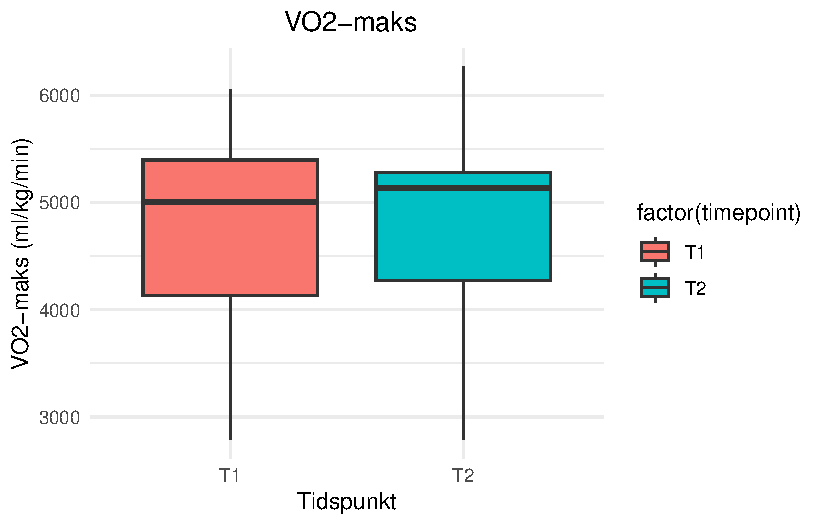
\includegraphics{01-reliabilitet_files/figure-pdf/unnamed-chunk-2-1.pdf}

}

\caption{\emph{\textbf{Figur 1:} Boksplot av VO2-maks på testdag 1 (T1)
og testdag 2 (T2).}}

\end{figure}

\begin{figure}

{\centering 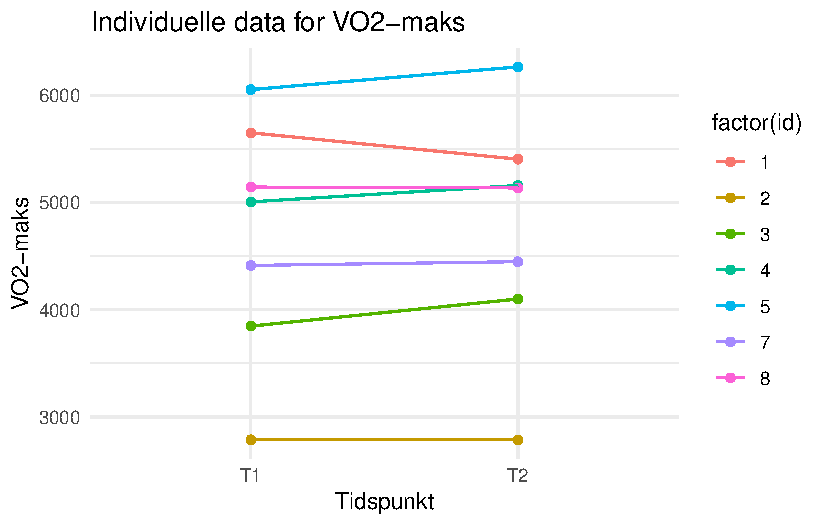
\includegraphics{01-reliabilitet_files/figure-pdf/unnamed-chunk-3-1.pdf}

}

\caption{\emph{\textbf{Figur 2:} Figuren viser VO2-maks målinger fra
testdag 1 (T1) til testdag 2 (T2).}}

\end{figure}

\begin{longtable}[]{@{}
  >{\raggedright\arraybackslash}p{(\columnwidth - 10\tabcolsep) * \real{0.2571}}
  >{\raggedleft\arraybackslash}p{(\columnwidth - 10\tabcolsep) * \real{0.1857}}
  >{\raggedleft\arraybackslash}p{(\columnwidth - 10\tabcolsep) * \real{0.2000}}
  >{\raggedleft\arraybackslash}p{(\columnwidth - 10\tabcolsep) * \real{0.1143}}
  >{\raggedleft\arraybackslash}p{(\columnwidth - 10\tabcolsep) * \real{0.1143}}
  >{\raggedleft\arraybackslash}p{(\columnwidth - 10\tabcolsep) * \real{0.1286}}@{}}
\caption{\emph{\textbf{Tabell 1:} Deltakernes karakteristika ved
oppstart (N = 7).}}\tabularnewline
\toprule\noalign{}
\begin{minipage}[b]{\linewidth}\raggedright
Variabel
\end{minipage} & \begin{minipage}[b]{\linewidth}\raggedleft
Gjennomsnitt
\end{minipage} & \begin{minipage}[b]{\linewidth}\raggedleft
Standardavvik
\end{minipage} & \begin{minipage}[b]{\linewidth}\raggedleft
Median
\end{minipage} & \begin{minipage}[b]{\linewidth}\raggedleft
Minimum
\end{minipage} & \begin{minipage}[b]{\linewidth}\raggedleft
Maksimum
\end{minipage} \\
\midrule\noalign{}
\endfirsthead
\toprule\noalign{}
\begin{minipage}[b]{\linewidth}\raggedright
Variabel
\end{minipage} & \begin{minipage}[b]{\linewidth}\raggedleft
Gjennomsnitt
\end{minipage} & \begin{minipage}[b]{\linewidth}\raggedleft
Standardavvik
\end{minipage} & \begin{minipage}[b]{\linewidth}\raggedleft
Median
\end{minipage} & \begin{minipage}[b]{\linewidth}\raggedleft
Minimum
\end{minipage} & \begin{minipage}[b]{\linewidth}\raggedleft
Maksimum
\end{minipage} \\
\midrule\noalign{}
\endhead
\bottomrule\noalign{}
\endlastfoot
Alder (år) & 24.14 & 2.18 & 24.00 & 22.00 & 29.00 \\
Høyde (cm) & 179.43 & 4.60 & 176.00 & 175.00 & 187.00 \\
Vekt (kg) & 77.64 & 7.97 & 79.20 & 60.60 & 88.90 \\
VO2-maks (ml/min) & 4729.43 & 1071.11 & 5072.00 & 2787.00 & 6266.00 \\
Watt-maks (W) & 421.43 & 82.54 & 437.50 & 275.00 & 525.00 \\
MAOD.a (\%) & 69.34 & 17.43 & 77.88 & 43.21 & 92.41 \\
\end{longtable}

\emph{\textbf{Notat:} Data er presentert som gjennomsittet,
standardavviket, median og minimums- og maksimumsverdi. VO2-maks =
maksimalt oksygenopptak; MAOD.a = maksimalt akkumulert
oksygenunderskudd.}

\begin{longtable}[]{@{}
  >{\raggedleft\arraybackslash}p{(\columnwidth - 12\tabcolsep) * \real{0.0417}}
  >{\raggedleft\arraybackslash}p{(\columnwidth - 12\tabcolsep) * \real{0.1389}}
  >{\raggedleft\arraybackslash}p{(\columnwidth - 12\tabcolsep) * \real{0.1111}}
  >{\raggedleft\arraybackslash}p{(\columnwidth - 12\tabcolsep) * \real{0.1250}}
  >{\raggedleft\arraybackslash}p{(\columnwidth - 12\tabcolsep) * \real{0.2083}}
  >{\raggedleft\arraybackslash}p{(\columnwidth - 12\tabcolsep) * \real{0.1806}}
  >{\raggedleft\arraybackslash}p{(\columnwidth - 12\tabcolsep) * \real{0.1944}}@{}}
\caption{\emph{\textbf{Tabell 2:} Utregning av variasjonskoeffisient
(\%) og standardavvik (N = 7).}}\tabularnewline
\toprule\noalign{}
\begin{minipage}[b]{\linewidth}\raggedleft
id
\end{minipage} & \begin{minipage}[b]{\linewidth}\raggedleft
cv\_vo2max
\end{minipage} & \begin{minipage}[b]{\linewidth}\raggedleft
cv\_wmax
\end{minipage} & \begin{minipage}[b]{\linewidth}\raggedleft
cv\_maoda
\end{minipage} & \begin{minipage}[b]{\linewidth}\raggedleft
std\_dev\_vo2max
\end{minipage} & \begin{minipage}[b]{\linewidth}\raggedleft
std\_dev\_wmax
\end{minipage} & \begin{minipage}[b]{\linewidth}\raggedleft
std\_dev\_MAODa
\end{minipage} \\
\midrule\noalign{}
\endfirsthead
\toprule\noalign{}
\begin{minipage}[b]{\linewidth}\raggedleft
id
\end{minipage} & \begin{minipage}[b]{\linewidth}\raggedleft
cv\_vo2max
\end{minipage} & \begin{minipage}[b]{\linewidth}\raggedleft
cv\_wmax
\end{minipage} & \begin{minipage}[b]{\linewidth}\raggedleft
cv\_maoda
\end{minipage} & \begin{minipage}[b]{\linewidth}\raggedleft
std\_dev\_vo2max
\end{minipage} & \begin{minipage}[b]{\linewidth}\raggedleft
std\_dev\_wmax
\end{minipage} & \begin{minipage}[b]{\linewidth}\raggedleft
std\_dev\_MAODa
\end{minipage} \\
\midrule\noalign{}
\endhead
\bottomrule\noalign{}
\endlastfoot
1 & 3.15 & 10.88 & 3.41 & 34.79 & 10.61 & 0.55 \\
2 & 0.03 & 6.15 & 4.51 & 0.14 & 3.54 & 0.73 \\
3 & 4.50 & 4.88 & 2.32 & 35.78 & 3.54 & 0.22 \\
4 & 2.13 & 11.47 & 7.68 & 21.64 & 10.61 & 1.26 \\
5 & 2.43 & 0.00 & 4.47 & 29.98 & 0.00 & 0.80 \\
7 & 0.56 & 0.00 & 2.22 & 4.95 & 0.00 & 0.23 \\
8 & 0.11 & 0.00 & 22.68 & 1.13 & 0.00 & 2.33 \\
\end{longtable}

\emph{\textbf{Notat:} Data er presentert variasjonskoeffisient (\%) og
standardavvik for hver av de tre utfallsvariablene for hver deltaker.
cv\_vo2max = variasjonskoeffisient (\%) for maksimalt oksygenopptak;
cv\_wmax = variasjonskoeffisient (\%) for watt-maks; cv\_maoda =
variasjonskoeffisient (\%) for maksimalt akkumulert oksygenunderskudd;
std\_dev\_vo2max = standardavvik for maksimalt oksygenopptak;
std\_dev\_wmax = standardavvik for watt-maks; std\_dev\_maoda =
standardavvik for maksimalt akkumulert oksygenunderskudd.}

\begin{longtable}[]{@{}lrr@{}}
\caption{\emph{\textbf{Tabell 3:} Gjennomsnittlig variasjonskoeffisient
(\%) og minste betydningsfulle forskjell (N = 7).}}\tabularnewline
\toprule\noalign{}
Variable & CV (\%) & SWC \\
\midrule\noalign{}
\endfirsthead
\toprule\noalign{}
Variable & CV (\%) & SWC \\
\midrule\noalign{}
\endhead
\bottomrule\noalign{}
\endlastfoot
VO2max & 1.84 & 18.34 \\
W.max & 4.77 & 4.04 \\
MAOD.a & 6.76 & 0.88 \\
\end{longtable}

\emph{\textbf{Notat:} Data er presentert som gjennomsnittlig
variasjonskoeffisient (\%) og minste betydningsfulle forskjell for hver
av de tre utfallsvariablene. VO2max = maksimalt oksygenopptak; W.max =
watt-maks; MAOD.a = maksimalt akkumulert oksygenunderskudd; CV =
variasjonskoeffisient; SWC = minste betydningsfulle forskjell. }

\hypertarget{metodisk-diskusjon}{%
\section{Metodisk diskusjon}\label{metodisk-diskusjon}}

Noen aspekter ved metoden kan i retrospekt ha vært suboptimale, og kan
følgelig ha påvirket validiteten til resultatene i negativ grad. Under
den submaksimale testen ble testdeltakerne bedt om å sykle på den samme
tråkkfekvensen som de ville sykle på under MAOD-testen. Ettersom
belastningen under den submaksimale testen er mye lavere enn under
MAOD-testen, kan tråkkfrekvensen oppleves kunstig høy under den
submaksimale testen, og følgelig føre til en dårlig arbeidsøkonomi. For
å fjerne feilkilden, kunne man ha individualisert hvilken watt den
enkelte testdeltaker syklet på under de submaksimale dragene, slik at
oksygenopptaket blir representativt for den gitte motstanden. Mengden
verbal tilbakemelding fra testleder til forsøksperson under VO2-maks- og
MAOD-testen kunne variere mellom T1 og T2. Dette kan skyldes at
testlederne var noe tilbakeholdne på T1, og ble mer selvsikre på T2.
Dette kan tenkes å ha påvirket testdeltakerne sin innsats i varierende
grad mellom T1 og T2. Flere av testdeltakerne hadde Wmaks som varierte
mye mellom første og andre testdag. Det regjerer således tvil om
LODE-sykkelen som ble benyttet under testingen samsvarte med den
motstanden vi stilte den inn på. Dette kan ha påvirket testresultatene.

\hypertarget{konklusjon}{%
\section{Konklusjon}\label{konklusjon}}

De fysiologiske testene viste varierende reliabilitet. Noen av testene
viste svært god reliabilitet for noen av forsøkspersonene, og dårlig
reliabilitet for andre. Vi konkluderte med at dette hovedsakelig
skyldtes at Lode-sykkelen hadde varierende motstand på en gitt watt. På
grunn av disse begrensningene, kan vi ikke være sikre på at en ny test
ville gi de samme resultatene som testene utført her. Fremtidige studier
bør se til at sykkelen har konsekvent motstand, individuelt tilpasse
watten på de submaksimale dragene og standardisere verbal
tilbakemelding.

\bookmarksetup{startatroot}

\hypertarget{labbrapport---ekstraksjon-og-analyse-av-protein}{%
\chapter{Labbrapport - ekstraksjon og analyse av
protein}\label{labbrapport---ekstraksjon-og-analyse-av-protein}}

\hypertarget{introduksjon}{%
\section{\texorpdfstring{\textbf{Introduksjon}}{Introduksjon}}\label{introduksjon}}

Proteiner gjør det meste av arbeidet i cellene i kroppen, og er
nødvendig for strukturen, funksjonene og reguleringen av kroppens vev og
organer. De er essensielle deler av organismen, og deltar praktisk talt
i alle prosesser i kroppen (Alberts et al. 2002). Det å kunne analysere
proteiner vil derfor være av stor betydning, og svært interessant å se
på innen ulike fagområder, som celle- og molekylærbiologi.

Det å studere protein og proteinkonsentrasjonen i muskelceller har blitt
brukt i flere treningsstudier {[}Hammarström et al. (2020); Stec et al.
(2016){]}. Den biologiske tilpasningen til motstandstrening varierer
mellom personer, på bakgrunn av variabler som treningsvolum, intensitet,
repetisjoner og frekvens av treningsøktene {[}American College of Sports
Medicine (2009){]}. I tillegg til at genetiske og epigenetiske
disposisjoner og miljøfaktorer spiller en rolle for variasjoner i
tilpasninger Timmons (2011). Ved å studere protein kan man se på blant
annet interaksjon, lokasjon og aktiveringsstatus av ulike proteiner.
Dette kan for eksempel brukes for å fremme gunstige
treningstilpasninger.

I denne labbrapporten har vi gjort en protein ekstraksjon og analyse. Én
frivillig person meldte seg til å ta en mikrobiopsi fra vastus
lateralis, i venstre og høyre bein. Personen gjennomførte eksentrisk
beinpress til utmattelse på venstre bein før prøvetaking. Vi var
interessert i å se på det fosforylerte p-70 proteinet til denne
personen, og forskjellen i konsentrasjonen mellom venstre og høyre bein.
Prøvene ble tatt på Høgskolen i Innlandet, 30.oktober 2023. Resterende
prøver som er analysert er hentet fra mikrobiopsi fra én trent- og én
utrent person. I denne analysen var vi interessert i å se på
UBF-proteinet, og sammenlikne konsentrasjonen av dette proteinet mellom
personene.

\hypertarget{teori}{%
\section{\texorpdfstring{\textbf{Teori}}{Teori}}\label{teori}}

Det er individuelle forskjeller på adaptasjoner til styrketrening, målt
i muskelstyrke og muskelmasse, og dette korrelerer med
muskelcelle-karakteristikker i hvile og under trening (Raue et al. 2012;
Stec et al. 2016; Terzis et al. 2008; Thalacker-Mercer et al. 2013).
Hemmelse av proteinet mTORC1 svekker proteinsyntesen hos mennesker
Drummond et al. (2009), mens aktivering av proteinet S6-Kinase 1
(S6K1/p-70), som ligger nedstrøms for mTORC1, gir en økning i
proteinsyntesen og påfølgende økning i muskelvekst Burd et al. (2010);
Terzis et al. (2008). Et økt treningsvolum vil føre til større
fosforylering av S6K1, og dermed markante tilpasninger gjennom gjentatte
episoder med økt proteinsyntese {[}Burd et al. (2010); Terzis et al.
(2010); Ahtiainen et al. (2015). Dette er grunnen til at vi ønsker å se
på konsentrasjonen av p-70 i det beinet som har trent til utmattelse,
mot det beinet som ikke har trent rett før prøvetaking.

Det er korrelasjon mellom mengden UBF-protein i cellene, og hastigheten
på ribosomal DNA-transkripsjon i hvilende og serum-stimulerte celler
(\textbf{glibetic1995?}). Mitotisk cellevekst krever kontinuerlig
ribosombiogenese, som er nødvendig for å støtte proteinsyntesen. Desto
raskere cellene går gjennom cellesyklusen, desto raskere må
ribosombiogenesen skje. Denne prosessen begrenses av hastigheten på
transkripsjonen av rRNA-genene (rDNA). Det betyr at dersom
konsentrasjonen av UBF i cellene er stor, vil transkripsjonen av rDNA gå
raskere. Dette er med på å styre produksjonen av ribosomer, og de er
essensielle for proteinsyntesen og cellevekst (\textbf{glibetic1995?}).
Dette er grunnen til at vi ønsker å se på konsentrasjonen av
UBF-proteinet i beinet til én trent person versus en utrent.

For å analysere de aktuelle proteinene ble det brukt en metode kalt
Western blot. Western blot er en immunologisk metode som brukes i celle-
og molekylærbiologi. Teknikken brukes for å separere og identifisere
spesifikke proteiner fra en kompleks blanding av proteiner ekstrahert
fra celler. I Western blot blir en blanding av proteiner separert basert
på molekylvekt og dermed type, gjennom gel-elektroforese. Resultatene
overføres deretter til en membran, som produserer et bånd for hvert
protein. Membranen inkuberes deretter med merkede antistoffer spesifikke
for det ønskede proteinet (\textbf{yang2012?}).

De ubundne antistoffene vaskes bort, slik at det kun er de bundne
antistoffene til proteinet som man er interessert i blir igjen. De
bundne antistoffene detekteres ved fremkalling av film. Siden
antistoffene bare binder seg ved de proteinene av interesse, skal kun
ett bånd være synlig. Tykkelsen på båndet samsvarer med mengden protein
som er til stede. Western blot er en nyttig teknikk proteindeteksjon der
man får muligheten til å kvantifisere proteinuttrykk
(\textbf{yang2012?}).

\hypertarget{metode}{%
\section{\texorpdfstring{\textbf{Metode}}{Metode}}\label{metode}}

\hypertarget{pruxf8vemateriale}{%
\subsubsection{\texorpdfstring{\textbf{Prøvemateriale}}{Prøvemateriale}}\label{pruxf8vemateriale}}

En frivillig på gruppa meldte seg til å ta en mikrobiopsi fra vastus
lateralis i både venstre og høyre ben. Vedkommende hadde trent styrke på
formiddagen, men gjennomførte 10 sett eksentriske benpress med venstre
fot til utmattelse. Derfor var vi interessert i å se på fosforylert p-70
protein. Resterende prøver vi analyserte var fra en mikrobiopsi fra en
trent person mens andre var fra en utrent person. Her var vi interessert
i å se på UBF-proteinet.

\hypertarget{oppsett-og-utgangspunkt-for-analyse}{%
\subsubsection{\texorpdfstring{\textbf{Oppsett og utgangspunkt for
analyse}}{Oppsett og utgangspunkt for analyse}}\label{oppsett-og-utgangspunkt-for-analyse}}

Til det vi gjorde i labben fikk vi ferdig behandlet muskelvev som var
fryst ned over natta. Western blot og bestemmelse av total
proteinkonsentrasjon ble gjort i motsatt rekkefølge, samt at prøven hvor
det ble bestemt total proteinkonsentrasjon var en vilkårlig tilgjengelig
prøve av tørt muskelvev som vi fikk utdelt.

Muskelbiopsien fra den frivillige ble homogenisert av bioingeniør som
beskrevet under metoden. Det ble ikke bestemt proteinkonsentrasjon, men
prøven ble også fortynnet i Laemmlibuffer (Bio-Rad) til å ha en
konsentrasjon på 1.5-2.0 µg/µl. Løsningen ble kokt i 5 min, 95 ℃. Kjølt
ned til romtemperatur og sentrifugert for å få ned kondens før vi
begynte på Western blot slik det er beskrevet.

\hypertarget{western-blot}{%
\subsubsection{\texorpdfstring{\textbf{Western
Blot}}{Western Blot}}\label{western-blot}}

Elektroforesekammeret ble lagt på is og fylt med buffer. Gelen vasket vi
med ultrarent vann (dH2O) før den ble lagt i kammeret. Tilsatte 5 µl
standard proteinstige, og 25 µl prøve (duplikat av hver) til gel etter
skjema. Alt vi tilsatte ble vortexet og sentrifugert før pipettering.
Satte i kjøleskap (4 ℃) og kjørte elektroforese i 30 min, 300 volt.

Demonterte gelen og la i overføringsbuffer med proteinside opp.
Membraner som proteinene skulle bli overført til klippet vi i ene
hjørnet og plasserte i methanol for å aktivere dem. Stod på shaker i
5-10 min. Våtgjorde 2 filterpapirer i overføringsbuffer og plassert oppå
gelen, snudde rundt og fjernet dem forsiktig sammen. Svamp som var
vasket med dH2O og hvor vannet var presset ut la vi i bunn i
monteringsbrett (svart side ned). Helte oppi overføringsbuffer og
plasserte filterpapiret med gel oppå svampen, fjernet eventuelle bobler.
Til slutt la vi membranen oppå gel, med svamp på toppen og lukket igjen.
La i overføringskammer som lå på is, fylte med overføringsbuffer og
satte spenning på konstant 100 volt i 30 min.

Neste steg var å sjekke om vi fikk overført proteiner til membran og
kutte overflødig membran. Dyppet membran raskt i dH2O, la i MemCode
sensitizer og satt på shaker i 2 min. Deretter la vi i MemCode
reversible stain, og på shaker i 1 min. Dyppet så raskt 3 ganger i
MemCode destain og ristet litt for å få det til å dekke membranen.
Dekket membran med methanol/destain-løsning (blandet 1:1) og satte på
shaker i 5 min. Skylte med dH2O før vi tok bilde av membraner. Fortsatte
med å legge i eraser/methanol-løsning (blandet 1:1), på shaker i 10 min.
Vasket 4 ganger med dH2O og kuttet membranen etter hvilke brønner vi
hadde brukt. La over i TBS for lagring.

Deretter blokkerte vi membranen med melkeproteiner på de stedene hvor
det ikke allerede er proteiner. La membran i blokkeringsløsning (2.5 \%
melk blandet med TBS-T) i 1 time i romtemperatur på shaker. Før vi helte
ut blokkeringsløsningen og renset i TBS. Primær antistoffet som ble
brukt tilsatte vi oppi en løsning (5 \% melk i TBS-T), før vi inkuberte
membraner i løsningene over natten i 4 ℃. Antistoffene er fortynnet
1:200 i melkeløsningen. Prøvene fra høyre og venstre bein til den
frivillige fra gruppa ble lagt i p-70 antistoff fra 2.november. Mens de
andre to prøvene vi hadde fra en trent og en utrent person i et annet
prosjekt ble lagt i UBF-antistoff fra 2017 (t-UBF).

Neste dag vasket vi for primærantistoff før vi tilsatte sekundær
antistoff. Vasket med TBS-T, 2 x 1 min + 3 x 5 min på shaker. Tilsatte
sekundær antistoff (anti-mouse igG) til 2.5 \% melk/TBS-T-løsning, i
forholdet 1:3000. Brukte to ulike produsenter, membranen med p-70 primær
antistoff ble lagt i anti-mouse igG fra Cell signaling, mens resterende
i antistoff fra Thermo Fisher. Stod på vippebrett i 1 time i
romtemperatur. Etterpå vasket vi med TBS, 4 x 5 min på shaker. Inkuberte
membranen i ECL-løsning i 5-10 min, la den på platen for å ta bilde.

\hypertarget{homogenisering-av-muskelvev}{%
\subsubsection{\texorpdfstring{\textbf{Homogenisering av
muskelvev}}{Homogenisering av muskelvev}}\label{homogenisering-av-muskelvev}}

Tørr muskelprøve veies, brukte 1.88 mg tørrvekt. Tilsatte
protease/phosphatase inhibitorer til en iskald lysis buffer (Hepes
buffer), 500 µl Hepes buffer og 5 µl inhibitorer. Viktig at prøven var
på is til vi tilsatte Hepes buffer. Tilsatte 150 µl av blandingen til
muskelprøven knuste mekanisk for hånd. Mos til det ikke er noen synlige
biter igjen, første gang gikk det 20-30 sek før den ble satt på is
igjen. Plasser på SB2 rotator i kjøleskap og roterte prøve i 30 min.
Spinn den i 10 min på 10 000 g, 4 ℃, før vi forflyttet supernatanten
forsiktig til et nytt rør uten å forstyrre pelleten. Brukte ufortynnede
prøver, men resultatene var over maksimal konsentrasjon. Derfor
fortynnet vi med dH2O og bestemte total proteinkonsentrasjon på en 1:1
fortynning. Konsentrasjonen bestemte vi med Bradford Assay, brukte 10 µl
prøve + 250 µl reagent i hver brønn (Pierce Detergent Compatible
Bradford Assay Reagent, Thermo Fisher Scientific).

\hypertarget{resultater-1}{%
\section{\texorpdfstring{\textbf{Resultater}}{Resultater}}\label{resultater-1}}

Mengden fosforylert p-70 var større i venstre bein enn i høyre bein, se
Figure~\ref{fig-figur1}. Når det gjaldt homogeniseringen var det en god
korrelasjon mellom signal og konsentrasjon i kontrollene og prøvene (se
Figure~\ref{fig-figur2}). Gjennomsnittlig variasjonskoeffisient på
signalstyrken for kontrollene var 1.7, fremstilt i
Table~\ref{tbl-tabell1}. Det ble funnet en 350 \% større signalstyrke
for p-70 i venstre bein versus høyre bein. Høyre bein hadde en
signalstyrke på 2758 og 4842 (gjennomsnitt = 3800), mens venstre bein
hadde en signalstyrke på 14826 og 11793 (gjennomsnitt = 13309).
Homogeniseringen av de andre prøvene viste at 99,9 \% av variasjonen i
signal kunne forklares av konsentrasjon, og at signalstyrken for
proteinmengden var på 2,532, 2,166 og 2,454, henholdsvis. I tillegg
viste homogeniseringen akseptabel reliabilitet (variasjonskoeffisient
{[}CV{]} = 20 \%).

\newpage

\begin{figure}

{\centering 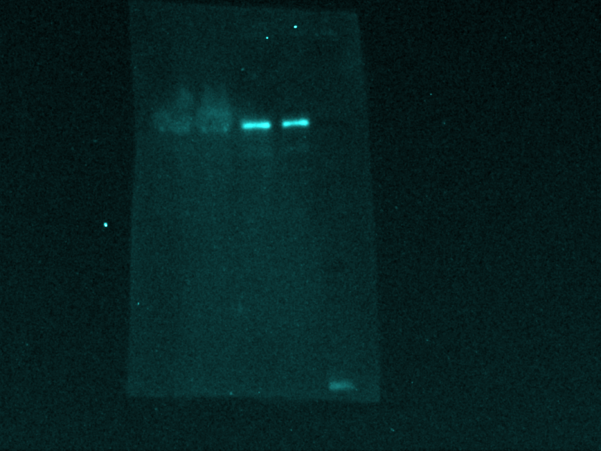
\includegraphics{figur1_analysert_bilde_p70.PNG}

}

\caption{\label{fig-figur1}\emph{Illustrasjon av mengden fosforylert
p-70 i venstre versus høyre bein. De to boksene til venstre viser mengde
p-70 i høyre fot og de to boksene til høyre viser mengde p-70 i venstre
fot (N = 1).}}

\end{figure}

\newpage

\begin{figure}

{\centering \includegraphics{figur2_spredningsplot_trendkurve.PNG}

}

\caption{\label{fig-figur2}\emph{Spredningsplott med trendkurve, som
illustrerer den forklarte variansen mellom signal og konsentrasjon (N =
1). Notat: Data er presentert som bestemmelseskoeffisient (R}2) (skala:
0,0--1,0).}

\end{figure}

\begin{figure}

{\centering \includegraphics{innsamlet-data/bilder/figur2_spredningsplot_trendkurve.png}

}

\caption{\emph{Spredningsplott med trendkurve, som illustrerer den
forklarte variansen mellom signal og konsentrasjon (N = 1). Notat: Data
er presentert som bestemmelseskoeffisient (R}2) (skala: 0,0--1,0).}

\end{figure}

\newpage

\hypertarget{tbl-tabell1}{}
\begin{longtable}{lr}
\caption{\label{tbl-tabell1}\emph{Tabellen viser resultatene fra homogeniseringen for bestemmelse av
proteinkonsentrasjon. CV er utregnet variasjonskoefisient for alle
kontrollene og prøven. Alle verdiene er beregnet basert på triplikat.
Pipetterte 3 av hver kontroll (A-H) og av prøveresultatene (P1).} }\tabularnewline

\toprule
 & cv (\%) \\ 
\midrule\addlinespace[2.5pt]
A & $2.27$ \\ 
B & $0.96$ \\ 
C & $3.75$ \\ 
D & $1.64$ \\ 
E & $1.12$ \\ 
F & $2.77$ \\ 
G & $1.04$ \\ 
H & $0.19$ \\ 
P1 & $8.09$ \\ 
\bottomrule
\end{longtable}

\hypertarget{diskusjon}{%
\section{\texorpdfstring{\textbf{Diskusjon}}{Diskusjon}}\label{diskusjon}}

\hypertarget{homogenisering}{%
\subsection{\texorpdfstring{\textbf{Homogenisering}}{Homogenisering}}\label{homogenisering}}

Den relativt høye, men akseptable, CV-en fra homogeniseringen kan
indikere en betydelig grad av variasjon i resultatene, noe som kan være
problematisk for reliabiliteten av eksperimentet. En potensiell årsak
til denne relativt høye CV-en kan være utvanningen av testløsningen som
vi var nødt til å utføre for å komme innenfor målegrensen for vårt
analyseapparat. Utvanning kan introdusere usikkerhet og øke variasjonen
i resultatene, spesielt når det gjelder prøver med lave konsentrasjoner
av målproteiner. Det er også verdt å merke at bruk av pipettespissen for
å blande løsningen kan ha ført til absorpsjon av vann eller proteiner,
og dette kan ha påvirket nøyaktigheten av målingene. Fremtidige
eksperimenter bør derfor vurdere alternative metoder for utvanning og
prøveblanding for å minimere denne typen feilkilder. Imidlertid er det
verdt å merke seg at bestemmelseskoeffisienten indikerer at selve
pipetteringen var vellykket, og dette gir en viss grad av tillit til
nøyaktigheten av våre målinger.

\hypertarget{western-blot-1}{%
\subsection{\texorpdfstring{\textbf{Western
blot}}{Western blot}}\label{western-blot-1}}

Western Blotting stiller høye krav til presisjon fra forskerne
(\textbf{ghosh2014?}). Dette gjør at marginale feil, som feil mengde
primærantistoff, kan føre til ugyldige resultater (\textbf{ghosh2014?}).
Videre har inter-forsker variabilitet vist seg å være den største
feilkilden, og kan utgjøre opptil 80 \% av den totale variasjonen
(\textbf{koller2005?}). På tross av alle disse potensielle feilkildene,
oppnådde vi adekvate resultater for p-70. Dette kan skyldes grundig
planlegging og nøye utførelse av western blotting-prosedyren. Selv om
teknikken stiller høye krav til presisjon fra forskerne, ble potensielle
feilkilder adressert gjennom en nøyaktig tilnærming til hver fase av
eksperimentet.

Muskelbiopsien resulterte derimot i ugyldige resultater for UBF. Dette
kan skyldes problemer med antistoffet (2017 årgang) (spesifisitet,
selektivitet eller reproduserbarhet), bufferløsningen eller antigenet
(\textbf{porstmann1985?}). Imidlertid fikk gruppe 4, som hadde et annet
antistoff (2022 årgang), heller ikke gyldige resultater for UBF. Dette
kan indikere at antistoffet potensielt ikke var hovedårsaken til de
ugyldige resultatene. Det bør likevel nevnes at kan settes spørsmålstegn
ved konsistensen til antistoffet til gruppe 4, dermed kan vi ikke
fullstendig utelukke at antistoffet kan ha bidratt til de ugyldige
resultatene for UBF.

En annen forklaring på de ugyldige resultatene kan være at mengden
antigen på membranen potensielt ikke har vært tilstrekkelig, da dette
også kan gi svakt eller ingen proteinsignal (\textbf{sule2023?}).
Proteiner som er uttrykt ved lave nivåer er mer sannsynlig å kreve en
lengre overføringstid eller en større mengde prøve (Mishra et al. 2019).
Imidlertid modifiserte vi ikke verken overføringstiden eller mengden
prøve. Dette kan dermed forklare deler av grunnen til at muskelbiopsien
resulterte i ugyldige resultater for UBF. Fremtidige eksperimenter bør
derfor vurdere å modifisere overføringstiden og prøvemengden ved
mistanke om utilstrekkelig antigen på membranen.

\bookmarksetup{startatroot}

\hypertarget{vitenskapsfilosofi}{%
\chapter{Vitenskapsfilosofi}\label{vitenskapsfilosofi}}

Jeg har valgt oppgave 1 og 2. Jeg skal ta for meg Humes argumentasjon
mot induksjon, samt se på om det er mulig å unngå hans konklusjon.
Videre skal jeg gi en kort beskrivelse og forklaring av
falsifikasjonisme. Til slutt vil jeg presenter ett problem med denne
teorien, og se på om dette problemet kan løses?

Hume (1711--1776) var en empirist. Han mente at kunnskap skal ha opphav
i erfaring gjennom sansene: syn, hørsel, berøring, lukt og smak. Hume
mente at alle forestillinger bare er en samling av inntrykk. Han var en
av de første til å kritisere induksjon. Induksjon er tankeprosess der vi
drar slutninger fra minner og erfaringer fra fortiden. Hume var spesielt
opptatt av hvordan man kan finne argumenter for å generalisere kunnskap
fra det man har observert til det uobserverte. Et eksempel på induksjon
er ravneparadokset, som er en observasjonsbasert bekreftelse av ulike
påstander: Ravn 1 er sort, ravn 2 er sort, ravn 3 er sort osv. Altså er
alle ravner sorte (Hempel 2000). Hume gir oss generelle grunner til å
tro at denne formen for slutning ikke har noe rasjonelt grunnlag. Humes
poeng er at vi ikke engang kan si at premissene sannsynliggjør
konklusjonen uten å anta at fremtiden vil ligne fortiden, og dette er en
antagelse vi ikke kan begrunne.

Hume mente at ettersom fremtiden ikke er nåtiden har man ikke erfart det
enda, og hvis man ikke har erfart det er det ikke sikker viten. Han
setter det på spissen ved å hevde at selv om solen har stått opp hver
eneste morgen hittil, kan man ikke vite sikkert at solen vil stå opp i
morgen. F.eks. Solen har stått opp hver dag i hittil, derfor kommer den
til å stå opp i morgen. På hvilket grunnlag kan vi si at dette er sant?
Tidligere erfaring. Hvordan gir fortiden oss grunn til å mene og tro noe
om fremtiden? Fremtiden vil være som fortiden, i morgen kommer til å
ligne på i dag, altså solen vil stå opp i morgen også. Hvordan vet vi
dette? Fordi det har alltid tidligere skjedd. Hele denne slutningen
faller på seg selv i en sirkelargumentasjon. Induksjon er dermed ikke en
logisk gyldig slutning. At fremtiden vil være som fortiden kan man se er
en skjult antagelse ved å sjekke hva som skjer med argumentet hvis man
gjør en annen antagelse. F.eks. «Fremtiden vil være helt forskjellig fra
fortiden». Derfor er «Fremtiden vil være som fortiden» et skjult
premiss.

Hume sier at vi ikke kan rasjonelt begrunne uniformitetsprinsippet (UP).
Han mener mange ender opp med å tro, på kun av vane, og at alle årsaker
dermed vil føre til like virkninger som vi har erfart i fortiden og
nåtiden (Bøhn and Gjelsvik 2015). Her er en idé som i utgangspunktet ser
ut til å være fornuftig: 1) UP har alltid vært sann tidligere, 2) UP er
sann nå, 3) derfor vil UP være sann i fremtiden. Dette argumentet er
altså sirkulært, og det finnes ikke noe ikke-sirkulært argument for UP.
Hume mente videre at det ikke er noe rasjonell begrunnelse for UT, det
kan ikke bevises gjennom logikk, og man kan ikke sjekke om det er sant.
UP er altså bare noe man må anta uten begrunnelser. Humes argument blir
da: 1) Hvert induktivt argument forutsetter UP, 2) UP har ingen rasjonal
begrunnelse, 3) derfor har konklusjonen av alle induktive argumenter
ingen rasjonal begrunnelse.

Selv om Hume har vist at vi ikke kan være sikre på at årsaker vil føre
til lik virkning i nåtiden som vi har erfart i fortiden, er mange av
våre overbevisninger rasjonelt begrunnet uten at vi er helt sikre på om
de er sanne. I tillegg til at vi ikke kan være sikre på hva som kommer
til å skje, gitt det som har skjedd tidligere, er Hume poeng at
sannsynlighetspåstander også forutsetter uniformitetsprinsippet. For
eksempel kan vi ikke utlede at solen vil stå opp i morgen fra prinsipper
om fortiden, men sannsynligheten for at det skjer. Hvis man skal avvike
fra UP, bør man ha en konkret grunn til å gjøre det. Og det har vi.
Fysikkens og kjemiens lover har ikke endret seg, de er de samme i fortid
og nåtid. Det vil derfor blant annet si at jern vil, også i fortiden,
ruste til rødfarge i kontakt med oksygen, bølgemerker vil fortsatt
dannes langs strendene og kull vil avsettes i sumpområder så lenge det
finnes planter her.

Falsifiseringsprinsippet er knyttet til Karl Popper (1902--1994). Han
mente at Humes induksjonsproblem ikke kunne løses, og at induktiv logikk
er et mislykket prosjekt. Ifølge Popper er det å lete etter bekreftelser
på hypoteser faktisk kjennetegn på pseudovitenskap. Han hevdet at
verifikasjon ikke hadde noen rolle i vitenskap i det hele tatt, men at
all vitenskap er nødt til å være falsifiserbar. Om teorien blir
verifisert, som betyr bekreftes, eller falsifisert vil det ha påvirkning
på teoriens validitet (gyldighet). Selv om teorien verifiseres, er det
ifølge Popper enda ikke gitt at teorien stemmer.

Avgrensningsproblemet til Popper var å skille vitenskap fra
ikke-vitenskap. Ved å si at S er en vitenskapelig påstand hvis og bare
hvis S er falsifiserbar ble hans løsning på avgrensningsproblemet. Her
kan vi ta ravneparadokset som et eksempel igjen. Påstanden om at alle
ravner er svarte (Hempel 2000). Denne påstanden kan aldri verifiseres,
fordi da må vi vite at alle ravner, i hele verden, til enhver tid har
vært svarte. Derimot kan den falsifiseres ved å se én ravn med en annen
farge enn svart. Man må merke seg at et utsagn kan være falsifiserbart
uten å være usant, for eksempel kan et objekt være vannløselig uten
faktisk oppløsning. Videre må man se opp for følgene feil som blander
sammen folk og påstander. Selv om folk som tror teori T er uvillige til
å gi opp sin tro uansett hva bevisene er, er ikke teori T falsifiserbar.
Tenk her på falsifiserbare uttalelse som «Jorden er flat» eller «Månen
er helt rund». Det faktum at det er flat jord eller rund måne viser ikke
at teorien ikke er falsifiserbar. Man må også merke seg at det er flere
grader av falsifisering. En teori eller uttalelse er mer falsifiserbar
enn en annen hvis den innebærer mer presise eller flere prediksjoner.

Gjennom falsifikasjon av en teori vil man aldri kunne gi den status som
endelig og korrekt, da den plutselig en dag kanskje vil vise seg å være
falsifisert ved en etterprøving av teorien, altså være feil. Selv om en
teori er utprøvd uendelig mange ganger, og aldri blitt falsifisert, kan
en ikke si at den er verifisert, da dette ikke er logisk gyldig å si.
Man må leve med at de teoriene vi har er gjenstand for forbedring og
utbytting. I den forstand kan man aldri oppnå sikker viten. Poppers svar
på dette var at slike teorier er «korroborert» selv om de ikke er
bekreftet. Med bekreftelse mente han at det er empirisk evidens som
viser at teorien er sann og med korroborasjon mente han at teorien har
overlevd mange tidligere tester.

Avslutningsvis kan man likevel si at det er noen mangler og
feilslutninger i både Humes og Poppers teorier som gjør at de bør ses
som rettesnorer heller enn absolutte sannheter (Malnes 2018). Induksjon
kan være nyttig i det daglige liv på tross av dens mangler på rent
logisk grunnlag. Falsifisering i praksis vil si at en sterk teori kan
komme til å bli forkastet til fordel for en svakere teori. Det bør være
mulig å tilbakevise teorier i tidlig stadium, ettersom alle gode studier
utvikles over lang tid. Med studier følger det også noen
tilleggsantagelser, som for eksempel et måleinstrument som ikke stemmer.
Feil ved måleinstrumentet kan da føre til at en hypotese, på feil
grunnlag, kan bli forkastet. Men når det kommer til vitenskapen er det
klart at falsifikasjon virkelig har noe for seg fremfor verifikasjon.

\bookmarksetup{startatroot}

\hypertarget{studiedesign}{%
\chapter{Studiedesign}\label{studiedesign}}

\hypertarget{innledning}{%
\section{Innledning}\label{innledning}}

I denne oppgaven tar jeg sikte på å evaluere styrker og svakheter ved
metodiske tilnærmingen til fem studier som har undersøkt effekten av
styrketrening med daglig bølgeperiodisering på muskelhypertrofi. Basert
på styrkene og svakhetene ved de fem studiene, vil jeg avslutningsvis
komme med anbefalinger for fremtidige studier. De fem studiene som blir
vurdert inkluderer Buford et al. (2007), Lima et al. (2012), Foschini et
al. (2010), Harries, Lubans, and Callister (2016) og Kok, Hamer, and
Bishop (2009).

\hypertarget{styrker-og-svakheter-ved-studiene}{%
\section{Styrker og svakheter ved
studiene}\label{styrker-og-svakheter-ved-studiene}}

\hypertarget{studiedesign-1}{%
\subsection{Studiedesign}\label{studiedesign-1}}

Studiene til Buford et al. (2007), Lima et al. (2012), Foschini et al.
(2010), Harries, Lubans, and Callister (2016) og Kok, Hamer, and Bishop
(2009) har, som all forskning, alle sine styrker og svakheter. For det
første, Buford et al. (2007), Lima et al. (2012), Foschini et al.
(2010), Harries, Lubans, and Callister (2016) benyttet randomisering og
kontrollgrupper i sine studier. Dette er en vesentlig styrke, da
randomisering bidrar til å minimere bias og øker validiteten til
resultatene (Patil 2023). En randomisert tildeling av deltakere til
treningsgruppene bidrar til å sikre at deltakerne i de ulike gruppene er
sammenlignbare ved studiens begynnelse, og eventuelle systematiske
forskjeller mellom gruppene blir mindre sannsynlige (Patil 2023). I
tillegg gir tilstedeværelsen av en kontrollgruppe muligheten til å
kvantifisere effekten av daglig bølgeperiodisering sammenlignet med
ingen trening. Dette gjør det mulig å isolere den spesifikke
innvirkningen av daglig bølgeperiodisering på muskelhypertrofi. I
motsetning til disse studiene, ble Kok, Hamer, and Bishop (2009) utført
uten randomisering og inkluderte ingen kontrollgruppe. Uten
randomisering er det en økt risiko for at deltakerne i de ulike
treningsgruppene kan ha systematiske forskjeller som påvirker
resultatene (Moher et al. 2012). Mangelen på en kontrollgruppe gjør det
også vanskeligere å skille mellom effekten av daglig bølgeperiodisering
og andre faktorer som kan påvirke muskelhypertrofi. Derfor har Kok,
Hamer, and Bishop (2009) betydelige begrensninger når det gjelder
randomisering og kontrollgrupper.

Når det gjelder målemetoder for å kvantifisere muskelhypertrofi,
benyttet Buford et al. (2007), Foschini et al. (2010) og Kok, Hamer, and
Bishop (2009) valide og reliable målemetoder. Buford et al. (2007) og
Kok, Hamer, and Bishop (2009) brukte ultralyd for å vurdere
muskeltykkelse, mens Foschini et al. (2010) benyttet BOD POD for å måle
fettfri masse. Disse målemetodene er anerkjent for sin validitet og
relabilitet når det gjelder vurdering av kroppssammensetning (Fields,
Goran, and McCrory 2002; Nijholt et al. 2017). Dette styrker tillitten
til resultatene fra disse studiene og gir et sterkere vitenskapelig
grunnlag for å vurdere effekten av daglig bølgeperiodisering på
muskelhypertrofi. På den annen side benyttet Lima et al. (2012) og
Harries, Lubans, and Callister (2016) mindre valide og reliable
målemetoder, inkludert hudfoldsmålinger og InBody, henholdsvis (Larsen
et al. 2021; Silva et al. 2009). Spesielt kan estimerte målemetoder, som
benyttet i Lima et al. (2012), øke usikkerhet i resultatene, da de er
mer sårbare for menneskelig feil og variasjon (Silva et al. 2009). Dette
svekker validiteten til resultatene i Lima et al. (2012) og Harries,
Lubans, and Callister (2016), ettersom målemetodene potensielt ikke har
vært reliable nok til å oppdage betydningsfulle endringer i muskelmasse.
Som følge av dette vet man ikke med sikkerhet om endringene i
muskelmasse skyldes muskelhypertrofi, eller tilfeldige målefeil.

Når det gjelder generaliserbarhet, hadde alle studiene begrensninger.
Både Buford et al. (2007), Lima et al. (2012), Foschini et al. (2010),
Harries, Lubans, and Callister (2016) og Kok, Hamer, and Bishop (2009)
hadde utfordringer knyttet til begrenset utvalgsstørrelse (n = 20--32)
og representativitet. Disse begrensningene gjør det utfordrende å
ekstrapolere funnene fra disse studiene til bredere befolkninger. Et
lite utvalg kan føre til at resultatene er mer sensitive for tilfeldige
variasjoner, og de kan være mindre representative for den generelle
befolkningen (H.-Y. Kim 2015). Studielengde var også en faktor som
begrenset forståelsen av effekten av daglig bølgeperiodisering på
muskelhypertrofi. Alle studiene, inkludert Buford et al. (2007), Lima et
al. (2012), Foschini et al. (2010), Harries, Lubans, and Callister
(2016) og Kok, Hamer, and Bishop (2009), hadde relativt korte
studielengder på 12--14 uker. Dette begrenser evnen til å vurdere
langsiktige effekter av daglig bølgeperiodisering på muskelhypertrofi.
Muskelhypertrofi er en prosess som utvikler seg over tid, og korte
studielengder kan gi begrenset innsikt i treningsmetodens langsiktige
innvirkning på muskelvekst (DeFreitas et al. 2011).

Oppfølging av kosthold er også en viktig faktor som påvirket studienes
validitet. Foschini et al. (2010) skiller seg fra de andre studiene ved
å inkludere en grundig beskrivelse av deltakernes kosthold. Dette er
viktig for å forstå effekten av treningen, da kostholdet kan ha en
betydelig innvirkning på muskelhypertrofi (Brad Jon Schoenfeld, Aragon,
and Krieger 2013). Imidlertid manglet de andre studiene, inkludert
Buford et al. (2007), Lima et al. (2012), Harries, Lubans, and Callister
(2016) og Kok, Hamer, and Bishop (2009), denne viktige informasjonen.
Uten en beskrivelse av kostholdet kan det være vanskelig å vurdere om
endringer i resultatene skyldes treningsmetoden alene eller eventuelle
endringer i deltakernes kosthold. Dette kan derfor betraktes som en
vesentlig svakhet ved studiene til Buford et al. (2007), Lima et al.
(2012), Harries, Lubans, and Callister (2016) og Kok, Hamer, and Bishop
(2009). Når det gjelder oppfølging av deltakerne etter avsluttet
intervensjon, er det viktig å belyse at ingen av de nevnte studiene,
inkludert Buford et al. (2007), Lima et al. (2012), Foschini et al.
(2010), Harries, Lubans, and Callister (2016) og Kok, Hamer, and Bishop
(2009), gjennomførte en systematisk oppfølging av deltakerne etter
avsluttet treningsperiode. Dette kan anses som en betydelig svakhet i
studiene, da det begrenser forståelsen av eventuelle langsiktige
effekter av daglig bølgeperiodisering på muskelhypertrofi.

Det er også viktig å merke seg at graden av oppfølging under
styrketreningen varierte mellom studiene. Buford et al. (2007), Lima et
al. (2012), Foschini et al. (2010), Harries, Lubans, and Callister
(2016) og Kok, Hamer, and Bishop (2009) inkluderte alle en form for
oppfølging under treningsperioden. Dette kan ha hatt en positiv
innvirkning på studiene ved å veilede deltakerne og sikre korrekt
utførelse av treningsprogrammet. Regelmessig oppfølging kan hjelpe
deltakerne med å opprettholde motivasjonen og engasjementet gjennom
studien. Det kan også bidra til å minimere frafall, noe som er viktig
for å opprettholde dataintegriteten og studiens validitet (Dettori
2011). Alle studiene, inkludert Buford et al. (2007), Lima et al.
(2012), Foschini et al. (2010), Harries, Lubans, and Callister (2016) og
Kok, Hamer, and Bishop (2009), inkluderte midt-tester som en integrert
del av testprotokollen. Disse midt-testene gav muligheten til å vurdere
tidlige endringer eller tilpasninger i muskelhypertrofi og bidro til å
gi en mer helhetlig forståelse av treningsmetodens effekter.
Inkluderingen av midt-tester kan derfor betraktes som en vesentlig
styrke ved disse studiene.

Foschini et al. (2010) er den eneste studien som inkluderte klare og
veldefinerte kriterier for eksklusjon av deltakere som ikke oppfylte
visse krav eller som ikke fullførte studien. Dette kan betraktes som en
styrke ved denne studien, da det bidrar til å opprettholde
datakvaliteten og redusere muligheten for skjevhet i resultatene.
Tydelige kriterier er nødvendig for å sikre at utvalget forblir homogent
og at eventuelle avvik fra studieprotokollen blir identifisert og
håndtert på en konsistent måte. Foschini et al. (2010) og Harries,
Lubans, and Callister (2016) er de eneste studiene som implementerte
blinding av testlederen. Dette metodiske tiltaket minimere risikoen for
subjektive påvirkninger på resultatene (Monaghan et al. 2021). Når
testledere er blinde for deltakernes tildeling til trenings- eller
kontrollgrupper, blir potensialet for at testlederen ubevisst behandler
deltakerne forskjellig redusert (Monaghan et al. 2021). Dette bidrar til
økt validitet av resultatene ved å sikre at eventuelle endringer i
målinger blir reflektert nøyaktig og upåvirket av testlederens
forventninger eller preferanser (Monaghan et al. 2021).

\hypertarget{statistiske-analyser-1}{%
\subsection{Statistiske analyser}\label{statistiske-analyser-1}}

Buford et al. (2007), Lima et al. (2012), Foschini et al. (2010),
Harries, Lubans, and Callister (2016) og Kok, Hamer, and Bishop (2009)
har alle valgt litt ulike tilnærminger til de statistiske analysene, og
alle deres tilnærminger har sine styrker og svakheter. Buford et al.
(2007) viste en grundig tilnærming til normalfordeling ved bruk av
Shapiro-Wilk-testen og sjekket homogenitet blant gruppene med Bartlett's
test. Deres bruk av toveis ANOVA med repeterte målinger var
hensiktsmessig for å evaluere endringer over tid og mellom gruppene
(H.-Y. Kim 2014). Effektstørrelser ble også beregnet, noe som gir
innsikt i klinisk relevans (Pripp 2017). Ved å inkludere
effektstørrelser oppnås en dypere forståelse av forskningsfunnene
(Sullivan and Feinn 2012). Mens statistisk signifikans gir informasjon
om hvorvidt sannsynligheten for at et funn skyldes tilfeldigheter
(Fethney 2010), gir effektstørrelsene en konkret måling av denne
forskjellen og dermed dens praktiske (kliniske) betydning (Hojat and Xu
2004). Denne holistiske tilnærmingen gir en mer informativ og anvendelig
tolkning av resultatene (Davis et al. 2021). Imidlertid var mangelen på
styrkeanalyse i denne studien en vesentlig svakhet, da dette kan ha
påvirke studiens evne til å oppdage statistisk signifikante effekter
(Pripp 2017). Lima et al. (2012) presenterte dataene tydelig med
gjennomsnitt og standardavvik, og de gjennomførte normalitetskontroll
ved hjelp av Shapiro-Wilk-testen. Deres bruk av ANOVA for repeterte
målinger og Student's t-test for uavhengige utvalg var passende (Mishra
et al. 2019). I tillegg ble relabiliteten vurdert ved hjelp av
intraklassekoeffisient. En svakhet her var derimot manglende
rapportering av detaljer fra normalitetskontrollen, og det er også verdt
å merke seg at det heller ikke her ble gjennomført en styrkeanalyse.

Foschini et al. (2010) presenterte også dataene tydelig med gjennomsnitt
og standardavvik, og de gjennomførte normalitetskontroll ved hjelp av
Shapiro-Wilk W-testen. De brukte passende statistiske tester, inkludert
Student's t-test og repeterte målinger ANOVA (Mishra et al. 2019), og de
rapporterte effektstørrelser. Bruken av Tukey's post hoc-test for
multiple sammenligninger var også hensiktsmessig (Lee and Lee 2018).
Igjen var en svakhet her mangelen på detaljer fra normalitetskontrollen,
samt fraværet av en styrkeanalyse. Harries, Lubans, and Callister (2016)
gjennomførte normalitetskontroll og bekreftet at variablene oppfylte
normalitetskriteriene. En styrke ved denne studien var anvendelsen av
lineære blandingsmodeller for å evaluere effektene av gruppe, tid, og
interaksjonen mellom gruppe og tid (Harrison et al. 2018).
Effektstørrelser ble også rapportert, og disse ble tolket ved hjelp av
Hopkins-skalaen (Will G. Hopkins 2004). En svakhet var imidlertid
manglende detaljer fra normalitetskontrollen, og også manglende
styrkeanalyse for å vurdere studiens evne til å oppdage signifikante
effekter. Kok, Hamer, and Bishop (2009) vurderte forskjeller mellom
gruppene ved hjelp av uavhengige t-tester, noe som var en passende
statistisk tilnærming (H.-Y. Kim 2019). De brukte også en 2 × 4
repeterte målinger ANOVA for å evaluere effekter over tid og mellom
grupper, noe som er hensiktsmessig i eksperimentelle design der det
ønskes å undersøke interaksjonen mellom to faktorer mens det
kontrolleres for de gjentatte målingene innen deltakere eller enheter
(Muhammad 2023). I tillegg rapporterte de effektstørrelser og
konfidensintervaller. Igjen var mangelen på detaljer fra
normalitetskontrollen en svakhet, i tillegg til manglende styrkeanalyse.

Samlet sett viser disse sammenligningene at alle studiene har styrker,
som inkluderer normalitetskontroll, passende statistiske tester og
rapportering av effektstørrelser. Dette gir et godt grunnlag for å
evaluere effekten av styrketrening med daglig bølgeperiodisering på
muskelhypertrofi. Imidlertid er det også svakheter som bør bemerkes.
Manglende detaljer om normalitetskontroll i flere av studiene begrenser
forståelsen av dataenes fordeling. Mangelen på kontroll for multiple
sammenligninger kan føre til falske positive funn (Lindquist and Mejia
2015). En gjennomgående svakhet er manglende gjennomføring av en
styrkeanalyse for å vurdere studienes evne til å påvise signifikante
effekter (Pripp 2017). Dette er en vesentlig begrensning, spesielt når
man vurderer studienes validitet (Pripp 2017).

\hypertarget{anbefalinger-for-fremtidige-studier}{%
\section{Anbefalinger for fremtidige
studier}\label{anbefalinger-for-fremtidige-studier}}

\hypertarget{studiedesign-2}{%
\subsection{Studiedesign}\label{studiedesign-2}}

For fremtidige studier som tar sikte på å undersøke effekten av
styrketrening med daglig bølgeperiodisering på muskelhypertrofi, er det
flere viktige aspekter å vurdere for å forbedre kvaliteten på
forskningen og få bedre innsikt i denne treningsmetoden. For det første
er det avgjørende å øke utvalgsstørrelsen i studiene. Større
utvalgsstørrelse vil bidra til økt statistisk styrke og
generaliserbarhet, og resultatene vil være mer representative for den
generelle befolkningen (Thomas, Nelson, and Silverman 2015).
Studielengden bør også utvides. Korte studielengder, som observert i
disse inkluderte studiene, gir begrenset innsikt i de langsiktige
effektene av daglig bølgeperiodisering på muskelhypertrofi. Derfor bør
forskere vurdere å inkludere studier med lengre varighet, eksempelvis
seks måneder eller ett år, for å kunne evaluere treningsmetodens
langsiktige innvirkning på muskelvekst. Dette vil gi en mer helhetlig
forståelse av hvordan daglig bølgeperiodisering kan påvirke muskelmasse
over tid. Inkludering av en adekvat kontrollgruppe er avgjørende for å
sammenligne effekten av daglig bølgeperiodisering med andre
treningsmetoder eller mangel på trening. Dette vil bidra til å
tydeliggjøre treningsmetodens spesifikke innvirkning på muskelhypertrofi
og gi en mer robust sammenligning mellom ulike treningsregimer.

Det er viktig å inkludere en detaljert beskrivelse og oppfølging av
deltakernes kosthold i studiene. Kostholdet er en vesentlig faktor som
kan påvirke resultatene, og en grundig beskrivelse vil bidra til en mer
helhetlig forståelse av treningsmetodens effekt på muskelhypertrofi
(Brad Jon Schoenfeld, Aragon, and Krieger 2013). Dette kan omfatte
informasjon om kaloriinntak, makronæringsstoffer, kosttilskudd og
eventuelle kostholdsmodifikasjoner som deltakerne kan ha gjennomført i
løpet av studien. Dette vil også gi muligheten til å vurdere om
endringer i kostholdet kan ha påvirket resultatene. Implementering av
blinding av testleder og randomisering av deltakere vil redusere bias i
resultatene, og dette bør derfor praktiseres for å forbedre validiteten
til studiene (Monaghan et al. 2021). Blinding kan bidra til å minimere
subjektive vurderinger og sikre objektive målinger av muskelhypertrofi,
mens randomisering bidrar til å forhindre systematisk skjevhet i
tildelingen av deltakere til treningsgrupper (Monaghan et al. 2021;
Patil 2023). Oppfølging av deltakerne etter intervensjonen er nødvendig
for å evaluere langsiktige effekter og eventuelle bivirkninger av daglig
bølgeperiodisering. Dette vil gi en mer helhetlig forståelse av
treningsmetodens påvirkning på deltakernes kroppssammensetning og helse.
I tillegg vil dette muliggjøre evaluering av deltakernes etterlevelse av
treningen etter avsluttet intervensjon, noe som kan gi ytterligere
informasjon om langtidseffekten av styrketrening med daglig
bølgeperiodisering på muskelhypertrofi.

Klare kriterier for eksklusjon bør etableres for å minimere potensiell
skjevhet og usikkerhet i resultatene. Dette vil bidra til å sikre at
deltakere som ikke er representative for populasjonen blir ekskludert
fra studiene. Kriteriene for eksklusjon bør være tydelige, objektive og
forhåndsdefinerte. Studier bør utføres på varierte populasjoner,
inkludert både utrente og trenede individer. Dette vil bidra til å
identifisere om daglig bølgeperiodisering har ulik effekt avhengig av
treningsstatus, og det vil gi en mer omfattende forståelse av hvordan
denne treningsmetoden kan tilpasses ulike målgrupper. For bedre innsikt
i hvordan effektene av daglig bølgeperiodisering utvikler seg over tid,
bør studiene inkludere midt-tester og flere oppfølgingstidspunkter i
sine design. Dette vil gi en mer nyansert forståelse av hvordan
muskelhypertrofi utvikler seg i løpet av en treningsperiode og vil
tillate forskere å identifisere eventuelle platåer eller endringer i
treningsresponsen over tid.

Disse anbefalingene kan hjelpe fremtidige studier med å forbedre
metodikken og gi mer valide og generaliserbare resultater når de
undersøker effekten av styrketrening med daglig bølgeperiodisering på
muskelhypertrofi. Gode vitenskapelige metoder er avgjørende for å bygge
en solid forståelse av treningsmetoder og deres virkninger på kroppen.
Ved å ta hensyn til disse anbefalingene i planleggingen og
gjennomføringen av fremtidige studier, kan forskere bidra til å styrke
kvaliteten og relevansen av forskningen på effekten av styrketrening med
daglig bølgeperiodisering på muskelhypertrofi. Dette vil føre til en
bedre forståelse av denne treningsmetoden og hvordan den kan tilpasses
ulike målgrupper for å oppnå ønskede resultater.

\hypertarget{statistiske-analyser-2}{%
\subsection{Statistiske analyser}\label{statistiske-analyser-2}}

Fremtidige studier bør følge bestemte retningslinjer for å sikre at
resultatene er valide og kan tolkes riktig. Det første trinnet er å
utføre normalitetskontroll ved hjelp av tester som Shapiro-Wilk eller
andre egnede metoder. Dette inkluderer rapportering av teststatistikk og
p-verdier. Normalitetskontroll er viktig fordi det validerer
forutsetningen om normalfordeling, som er avgjørende for mange
statistiske analyser. Videre er det nødvendig å gjennomføre en grundig
styrkeanalyse for å bestemme hvor mange deltakere som trengs for å
oppdage statistiske signifikante effekter. Dette øker studiens evne til
å trekke konklusjoner basert på de planlagte analysene (Pripp 2017).
Detaljer fra dataanalyseprosessen, inkludert normalitetskontroll, valg
av statistiske tester, signifikansnivå (alfa) og eventuelle justeringer
for multiple sammenligninger, bør også nøye rapporteres. Dette gir
leserne muligheten til å evaluere studiens metodologi grundig. Fortsett
med rapporteringen av effektstørrelser, for eksempel Cohen's d eller
Eta-kvadrat, da disse gir innsikt i den kliniske relevansen av
resultatene (Hojat and Xu 2004). Dette hjelper leserne med å forstå om
de observerte forskjellene er av praktisk betydning. Spesielt i
tilfeller med store utvalgsstørrelser, hvor resultatene har en tendens
til å oppnå statistisk signifikans, selv ved irrelevante effekter (Faber
and Fonseca 2014).

Hvis det er behov for å utføre post hoc-analyser for å sammenligne flere
grupper eller betingelser, bør det benyttes passende metoder som Tukey's
test eller Bonferroni-korreksjon for å kontrollere for type I-feil (Lee
and Lee 2018). Det bør også vurderes å inkludere relabilitetsanalyser,
som intraklassekorrelasjon, spesielt hvis dataene er samlet over tid.
Dette gir informasjon om konsistensen av målinger over ulike tidspunkter
(Koo and Li 2016). Anerkjent statistisk programvare som R, SPSS eller
JASP bør benyttes, og det bør inkluderes informasjon om versjoner og
innstillinger som ble brukt i analysen. Avslutningsvis bør det brukes
grafiske elementer som figurer og tabeller for å visuelt representere
resultatene på en klar og forståelig måte (Divecha, Tullu, and Karande
2023). Disse trinnene vil bidra til å sikre at fremtidige studier blir
utført og rapportert på en måte som gir valide og betydningsfulle
resultater.

\bookmarksetup{startatroot}

\hypertarget{analyse-av-repeterte-forsuxf8k}{%
\chapter{Analyse av repeterte
forsøk}\label{analyse-av-repeterte-forsuxf8k}}

\hypertarget{introduksjon-1}{%
\section{Introduksjon}\label{introduksjon-1}}

Skjelettmuskulaturen er avgjørende for å opprettholde en sunn livsstil
(Wolfe 2006), og fremmer vedlikehold og/eller økning i styrke og effekt
(Chalhoub et al. 2018; Hayashida et al. 2014). Den mest potente,
ikke-farmakologiske stimulansen som induserer muskelhypertrofi og styrke
er styrketrening (McKendry et al. 2021). Mekanisk drag og metabolsk
stress indusert av styrketrening antas å aktivere intramuskulære
signalveier, noe som fører til økt proteintranslasjonseffektivitet og
muskelhypertrofi over tid (Brad J. Schoenfeld 2010; Terzis et al. 2008).
Selv om muskelhypertrofi kan forklare noe av økningen i styrke og effekt
med styrketrening, antas nevrologiske adaptasjoner å spille en mer
sentral rolle (Dankel et al. 2017). Manipulering av
styrketreningsvariabler som intensitet (Wernbom, Augustsson, and Thomeé
2007), volum (Brad J. Schoenfeld, Ogborn, and Krieger 2017), frekvens
(B. Schoenfeld, Ogborn, and Krieger 2016), inter-sett pauser (McKendry
et al. 2016), kontraksjonstype (Ato et al. 2016) og tid under spenning
(Burd et al. 2012) kan endre den intracellulære signaleringen og
muskelproteinsyntesens respons på styrketrening (Bird, Tarpenning, and
Marino 2005). Derfor er det viktig å forstå hvordan manipulering av
styrketreningsvariabler kan maksimere muskelhypertrofi og maksimal
styrke for evidensbaserte praktiske anbefalinger (Heaselgrave, Mckendry,
and Smeuninx 2018).

En styrketreningsvariabel som antas å være av spesiell betydning for å
maksimere muskelhypertrofi og maksimal styrke er volum, definert som
produktet av sett × repetisjoner × motstand (dvs. belastningsvolum),
eller antall ukentlige sett per muskelgruppe (dvs. settvolum)
(Figueiredo, Salles, and Trajano 2018). Meta-analyser indikerer at
moderat til høyt ukentlig styrketreningsvolum kan fremkalle marginalt
større styrkeøkninger enn lavt ukentlig styrketreningsvolum (Grgic et
al. 2018; Ralston et al. 2017). Det optimale styrketreningsvolumet for å
maksimere muskelhypertrofi og styrke forblir imidlertid uklart
(Heaselgrave, Mckendry, and Smeuninx 2018). Flere potensielle
sammenhenger mellom styrketreningsvolum og muskelhypertrofi og maksimal
styrke har blitt postulert: (i) et dose-respons-forhold, hvor gradvis
økning i ukentlig styrketreningsvolum fører til en større økning i
muskelhypertrofi og maksimal styrke (Brad J. Schoenfeld, Ogborn, and
Krieger 2017), (ii) et invertert-U-forhold, der økende ukentlig
styrketreningsvolum utover en viss terskel negativt påvirker
muskelhypertrofi (Figueiredo, Salles, and Trajano 2018), (iii) ingen
sammenheng mellom ukentlig styrketreningsvolum og muskelhypertrofi eller
maksimal styrke (Mitchell et al. 2012; Ostrowski et al. 1997; R.
Radaelli et al. 2014). Til dags dato har forskning ikke klart å
identifisere det optimale styrketreningsvolumet per muskelgruppe for å
maksimere muskelhypertrofi og maksimal styrke. Videre har den
eksisterende forskningen fokusert på fysiologiske og nevrologiske
adaptasjoner til relativt lavt styrketreningsvolum (≤ 10--12 ukentlige
sett), og fremhever et klart behov for å undersøke dette forholdet ved
høyere ukentlige styrketreningsvolum (\textgreater{} 10--12 ukentlige
sett) (Carroll, Riek, and Carson 2001; Brad J. Schoenfeld, Ogborn, and
Krieger 2017).

Mangelen på å identifisere ukentlig dose av styrketreningsvolum for å
maksimere fysiologiske og nevrologiske adaptasjoner er også
sannsynligvis en konsekvens av nyanser i eksperimentelle design og
kontrolltiltak (Heaselgrave, Mckendry, and Smeuninx 2018). Eksempelvis
har flere tidligere studier blitt utført i små kohorter av styrketrente
individer (Aube et al. 2022; Brigatto et al. 2022; Heaselgrave,
Mckendry, and Smeuninx 2018; Brad J. Schoenfeld et al. 2019).
Ekstrapolering av meningsfulle tolkninger fra trente til utrente
individer er problematisk, ettersom utrente individer kan oppleve
nevrale modifikasjoner (Carroll, Riek, and Carson 2001) og en utvidet
muskelproteinsynteserespons på akutt styrketrening (Damas et al. 2015;
Tang et al. 2008; Wilkinson et al. 2008). I tillegg har viktige
kontrolltiltak som ernæringsinntak ofte blitt oversett i studier av
styrketreningsvolum og muskelhypertrofi og maksimal styrke (Heaselgrave,
Mckendry, and Smeuninx 2018). For å håndtere disse manglene er det behov
for strenge kontrollerte studier som undersøker forholdet mellom
styrketreningsvolum og muskelhypertrofi og maksimal styrke (Heaselgrave,
Mckendry, and Smeuninx 2018).

Derfor var formålet med denne studien å undersøke effekten av lavt
versus moderat settvolum på muskelhypertrofi og maksimal styrke på
utrente individer. På bakgrunn av tidligere forskning på utrente
(Amirthalingam T et al. 2017; Regis Radaelli et al. 2015) og trente
individer (Aube et al. 2022; Brigatto et al. 2022; Heaselgrave,
Mckendry, and Smeuninx 2018; Brad J. Schoenfeld et al. 2019), var vår
hypotese at moderat settvolum resulterer i signifikant større økning i
muskelhypertrofi og maksimal styrke enn lavt settvolum på utrente
individer.

\hypertarget{materialer-og-metoder-1}{%
\section{Materialer og metoder}\label{materialer-og-metoder-1}}

\hypertarget{studieoversikt}{%
\subsection{Studieoversikt}\label{studieoversikt}}

Intervensjonen besto av 12 uker med styrketrening for hele kroppen. Alle
deltakerne startet forsøket i løpet av september til november.
Benøvelser ble utført unilateralt for å tillate differensiering av
treningsvolumet innenfor hver deltaker. I henhold til dette ble de to
bena til hver deltaker tilfeldig tildelt å utføre styrketreningsøvelser
bestående av ett sett (lavt settvolum) og tre sett (moderat settvolum)
(dvs. hver deltaker utførte begge protokollene). Muskelstyrken ble
vurdert ved utgangspunkt og etter treningsintervensjonen. I tillegg ble
kroppssammensetning (fettfri masse) målt før og etter
treningsintervensjonen. Fra og med uke 6 utførte deltakerne en
kostholdsregistrering der de veide og loggførte kostholdsinntaket i fire
til fem påfølgende dager, inkludert en helgedag.

\hypertarget{deltakere}{%
\subsection{Deltakere}\label{deltakere}}

Totalt 41 mannlige og kvinnelige deltakere ble rekruttert til denne
studien. Inklusjonskriteriene var (i) røykfrie og (ii) alder mellom 18
og 40 år. Eksklusjonskriterier var (i) intoleranse mot lokalbedøvelse,
(ii) treningshistorikk med mer enn én ukentlig styrketreningsøkt i løpet
av de siste 12 månedene før intervensjonen, (iii) nedsatt muskelstyrke
på grunn av tidligere eller nåværende skade og (iv) inntak av
foreskrevet medisin som kan påvirke adaptasjonene til styrketreningen.
Under dataanalysene ble syv deltakere ekskludert på bakgrunn av at de
ikke fullførte ≥ 85 \% av de planlagte treningsøktene med årsaker som;
ubehag eller smerter i underekstremiteter under trening (n = 5), skade
som ikke er relatert til studien (n = 1) og manglende overholdelse av
studieprotokollen (n = 1). Alle inkluderte deltakere rapporterte
tidligere erfaring med idrettsaktiviteter (f.eks. lagsport, langrenn og
turn). Tjue deltakere rapporterte at de var engasjert i fysisk trening
på tidspunktet for påmelding (median antall økter per uke: 2, område:
0,5--4,0), hvorav 10 utførte sporadisk styrketrening, men ingen mer enn
én gang per uke. Deltakernes karakteristika er presentert i Tabell 1.

\hypertarget{tabell-1-deltakernes-karateristika-ved-oppstart-n-41.}{%
\subsubsection{Tabell 1: Deltakernes karateristika ved oppstart (N =
41).}\label{tabell-1-deltakernes-karateristika-ved-oppstart-n-41.}}

\begin{longtable}[]{@{}
  >{\raggedright\arraybackslash}p{(\columnwidth - 16\tabcolsep) * \real{0.2308}}
  >{\raggedright\arraybackslash}p{(\columnwidth - 16\tabcolsep) * \real{0.0769}}
  >{\raggedleft\arraybackslash}p{(\columnwidth - 16\tabcolsep) * \real{0.0330}}
  >{\raggedleft\arraybackslash}p{(\columnwidth - 16\tabcolsep) * \real{0.1538}}
  >{\raggedright\arraybackslash}p{(\columnwidth - 16\tabcolsep) * \real{0.0659}}
  >{\raggedleft\arraybackslash}p{(\columnwidth - 16\tabcolsep) * \real{0.1538}}
  >{\raggedright\arraybackslash}p{(\columnwidth - 16\tabcolsep) * \real{0.0659}}
  >{\raggedleft\arraybackslash}p{(\columnwidth - 16\tabcolsep) * \real{0.1429}}
  >{\raggedright\arraybackslash}p{(\columnwidth - 16\tabcolsep) * \real{0.0769}}@{}}
\toprule\noalign{}
\begin{minipage}[b]{\linewidth}\raggedright
Inkludert/Ekskludert
\end{minipage} & \begin{minipage}[b]{\linewidth}\raggedright
Kjonn
\end{minipage} & \begin{minipage}[b]{\linewidth}\raggedleft
n
\end{minipage} & \begin{minipage}[b]{\linewidth}\raggedleft
Alder, M (SD)
\end{minipage} & \begin{minipage}[b]{\linewidth}\raggedright
\end{minipage} & \begin{minipage}[b]{\linewidth}\raggedleft
Hoyde, M (SD)
\end{minipage} & \begin{minipage}[b]{\linewidth}\raggedright
\end{minipage} & \begin{minipage}[b]{\linewidth}\raggedleft
Vekt, M (SD)
\end{minipage} & \begin{minipage}[b]{\linewidth}\raggedright
\end{minipage} \\
\midrule\noalign{}
\endhead
\bottomrule\noalign{}
\endlastfoot
Ekskludert & female & 4 & 22.9 & (1.6) & 165.5 & (7.6) & 64.6 & (9.7) \\
Ekskludert & male & 3 & 24.3 & (1.5) & 189.0 & (4.6) & 88.2 & (22.4) \\
Inkludert & female & 18 & 22.0 & (1.3) & 167.7 & (6.9) & 64.4 &
(10.4) \\
Inkludert & male & 16 & 23.6 & (4.1) & 182.9 & (5.9) & 75.8 & (10.7) \\
\end{longtable}

Notat: Data er presentert som gjennomsnitt (standardavvik). n = antall;
M = gjennomsnitt; SD = standardavvik.

\hypertarget{etisk-godkjenning}{%
\subsection{Etisk godkjenning}\label{etisk-godkjenning}}

Alle deltakerne ble informert om potensielle risikoer og ubehag knyttet
til studien og ga sitt informerte samtykke før studieregistrering.
Studiedesignet ble forhåndsregistrert (ClinicalTrials.gov Identifier:
NCT02179307), godkjent av den lokale etiske komiteen ved Høgskolen i
Lillehammer, Institutt for idrettsvitenskap (nr. 2013-11-22:2) og alle
prosedyrer ble utført i henhold til Helsinki-erklæringen.

\hypertarget{styrketreningsprotokoll}{%
\subsection{Styrketreningsprotokoll}\label{styrketreningsprotokoll}}

Før alle treningsøkter utførte deltakerne en standardisert
oppvarmingsrutine bestående av (i) 5 min ergometersykling (Borgs skala:
12--14), etterfulgt av (ii) 10 repetisjoner hver av kroppsvektøvelse
(armhevinger med individuelt tilpasset «leverage», magebøyinger, rygghev
og knebøy) og (iii) ett sett med 10 repetisjoner på \textasciitilde50 \%
av én repetisjon maksimum (1RM) for hver styrkeøvelse.
Styrketreningsøvelsene for underekstremitetene ble utført i følgende
rekkefølge; unilateral benpress, lårcurl og benekstensjon, utført som
enten ett sett (lavt settvolum) eller tre sett (moderat settvolum) per
øvelse. Lavt settvolum ble utført mellom det andre og tredje settet av
protokollen for moderat settvolum. Etter øvelsene for
underekstremitetene, utførte deltakerne to sett med hver av følgende
øvelser; bilateral benkpress, nedtrekk og enten skulderpress eller
sittende roing (utført i alternerende økter). Pausene mellom settene var
på 90--180 s. Den relative motstanden ble gradvis økt gjennom
intervensjonen, og startet med 10RM de første 2 ukene, etterfulgt av 8RM
i 3 uker og 7RM i 7 uker.

For å tilpasse treningsprogrammet bedre til en deltakers daglige
timeplan, ble noen økter utført uten tilsyn. Gjennomsnittlig antall
overvåkede økter var 91 \% (standardavvik {[}SD{]} = 10 \%, område:
67--100 \%) av utførte økter. For å overvåke økter uten tilsyn, ble
deltakerne bedt om å føre detaljerte logger. Disse ble kontinuerlig
kontrollert av forskerne sammen med deltakerne for å sikre progresjon og
overholdelse av protokollen. Fra den niende treningsøkten hadde hver uke
(inneholdt tre treningsøkter) en økt med redusert relativ motstand,
tilsvarende 90 \% av forrige økt med samme antall repetisjoner.
Treningsøkter med maksimal innsats ble atskilt med minst 48 timer.
Treningsøkter med submaksimal innsats (90 \%) ble atskilt fra andre
økter med minst 24 timer. For å hjelpe til med umiddelbar restitusjon
ble det gitt en standardisert drink etter hver økt som inneholdt 0,15 g
kg−1 protein, 1,2 g kg−1 karbohydrater og 0,5 g kg−1 fett.

\hypertarget{muxe5ling-av-muskelstyrke}{%
\subsection{Måling av muskelstyrke}\label{muxe5ling-av-muskelstyrke}}

Maksimal styrke ble vurdert som 1RM i unilateral benpress. Testøkten for
hver øvelse startet med en spesifikk oppvarming bestående av 10, 6 og 3
repetisjoner på henholdsvis 50, 75 og 85 \% av forventet maksimum.
Deretter ble 1RM funnet ved å øke motstanden gradvis inntil vekten ikke
kunne løftes gjennom hele bevegelsbanen. Deltakerne ble bedt om å skyve
med maksimal innsats. For hver øvelse ble den høyeste motstanden som ble
forsøkt definert som 1RM. Hver deltaker fikk fire til seks forsøk. Ved
utgangspunkt ble vurdering av 1RM utført to ganger, atskilt med minst 4
dager. Den maksimale verdien oppnådd for hver test ble brukt i
etterfølgende analyse. Styrketesten ble atskilt med minst 48 timer fra
tidligere treningsøkter.

\hypertarget{kroppssammensetning-fettfri-masse}{%
\subsection{Kroppssammensetning (fettfri
masse)}\label{kroppssammensetning-fettfri-masse}}

For å undersøke endringer i muskelmasse før og etter
treningsintervensjonen, ble kroppssammensetning (fettfri masse) vurdert
ved hjelp av dual-energy X-ray absorptiometry (DXA) (Lunar Prodigy, GE
Healthcare, Oslo, Norge), i henhold til standard protokoll. Før
DXA-målingene ble deltakerne bedt om å faste i 2 timer og avstå fra
anstrengende fysisk aktivitet i 48 timer. To dager skilte den siste
styrketestøkten fra målingen av kroppssammensetning.

\hypertarget{statistiske-analyser-3}{%
\subsection{Statistiske analyser}\label{statistiske-analyser-3}}

All deskriptiv data er presenteres som gjennomsnitt (standardavvik
{[}SD{]}), med mindre annet er angitt. For å undersøke effekten av lavt
versus moderat settvolum på muskelhypertrofi og maksimal styrke, ble det
utført en lineær regresjonsanalyse, der den avhengige variabelen var
definert som differansen mellom gruppene. Resultatene ble presenterte
som estimat, standardfeil (SE) t-verdi, konfidensintervall (KI), p-verdi
og prosent. Nivået av statistisk signifikans ble satt til α = 0,05. All
dataanalyse ble gjort i R (R Core Team, 2023).

\hypertarget{resultater-2}{%
\section{Resultater}\label{resultater-2}}

Overholdelse av protokollen var 96 ± 5 \% av de foreskrevne 31 øktene
(område: 81--100 \%). Totalt sett resulterte 12 uker med styrketrening i
en gjennomsnittlig økning på 193 g (2,25 \%) i fettfri masse og 92,3 kg
(55,14\%) i maksimal styrke. Dette var innenfor forventet rekkevidde av
treningsinduserte endringer (Ahtiainen et al. 2016). Gruppen med moderat
settvolum økte i gjennomsnitt 123 g (73,9 \%) mer i fettfri masse enn
gruppen med lavt settvolum (SE = 56,14, t = 2,19, 95 \% KI: 8,6--237,0,
p = 0,036, Figur 1). I tillegg økte gruppen med moderat settvolum i
gjennomsnitt 7,82 kg (12,5 \%) mer i maksimal styrke enn gruppen med
lavt settvolum (SE = 3,31, t = 2,36, 95 \% KI: 1,1--14,6, p = 0,025,
Figur 2).

\begin{figure}

{\centering 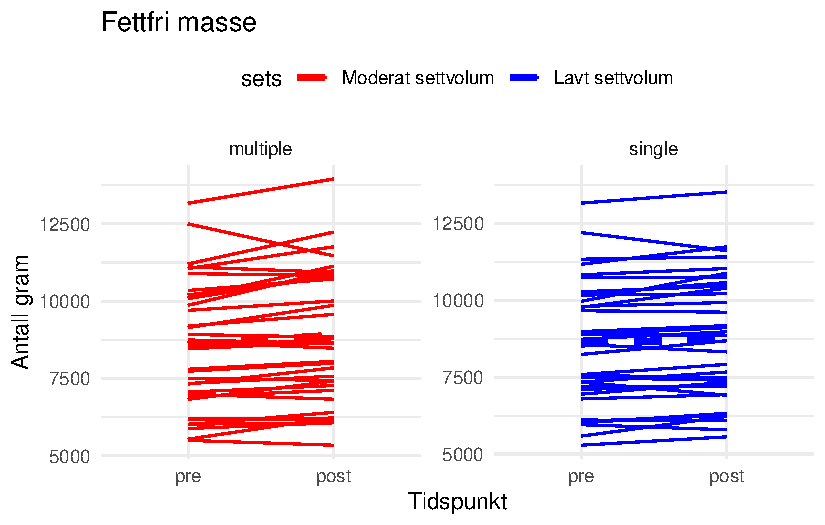
\includegraphics{05-analyse_av_repeterte_forsok_files/figure-pdf/Figur 1-1.pdf}

}

\caption{Figur 1: Endringer i fettfri masse ved lavt versus moderat
settvolum i løpet av en styrketreningsintervensjon på 12 uker (N = 34).
Notat: Stipplet linje = gjennomsnittlig respons; sammenhengende linje =
individuelle responser.}

\end{figure}

\begin{figure}

{\centering 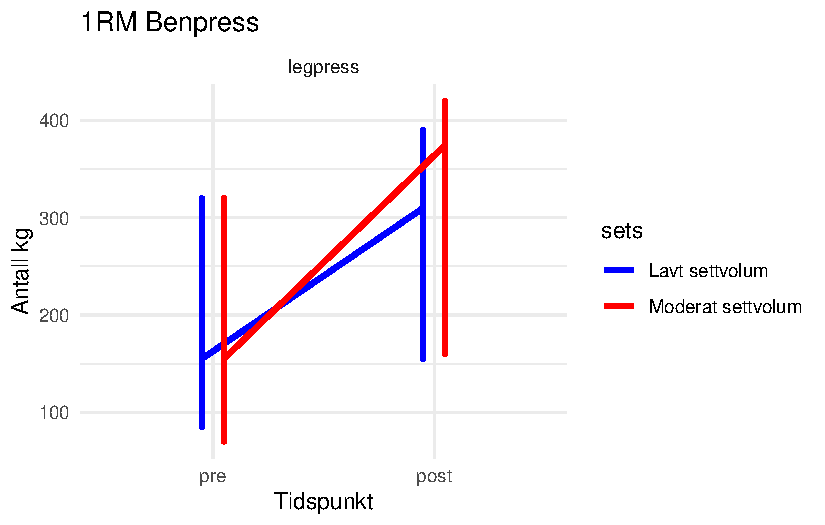
\includegraphics{05-analyse_av_repeterte_forsok_files/figure-pdf/Figur 2-1.pdf}

}

\caption{Figur 2: Endringer i maksimal styrke ved lavt versus moderat
settvolum i løpet av en styrketreningsintervensjon på 12 uker (N = 34).
Notat: Diagonale linjer = gjennomsnittlig respons; vertikale linjer =
minimums- til maksimumsverdi.}

\end{figure}

\hypertarget{diskusjon-1}{%
\section{Diskusjon}\label{diskusjon-1}}

Hensikten med denne studien var å undersøke effekten av lavt versus
moderat settvolum på muskelhypertrofi og maksimal styrke på utrente
individer. I samsvar med vår hypotese, fant vi at styrketrening med
moderat settvolum resulterte i signifikant større økning i
muskelhypertrofi og maksimal styrke enn lavt settvolum på utrente
individer. Dette er i tråd med resultatene fra tidligere meta-analyser
som konkluderte til fordel moderat, sammenlignet med lavt, settvolum for
muskelhypertrofi og maksimal styrke (Krieger 2009, 2010; Taylor et al.
2010; Brad J. Schoenfeld, Ogborn, and Krieger 2017).

Fra et mekanistisk perspektiv, selv om en rekke akutte studier har
rapportert assosiasjoner mellom mTORC1-mediert signalering av
muskelproteinsyntese og styrketreningsvolum ved \textasciitilde9
ukentlige sett (Burd et al. 2012; Terzis et al. 2010), er det evidens på
et platå i dette forholdet ved høyere styrketreningsvolum (dvs.
\textasciitilde24 ukentlige sett). Eksempelvis observerte Tibana et al.
(2017) en nedregulering i ekspresjonen av en rekke essensielle proteiner
implisert i muskelproteinsyntesen etter 24 versus 12 ukentlige sett per
muskelgruppe hos gnagere. I studien vår gjennomførte deltakerne i
gruppen med moderat styrketreningsvolum 12--18 ukentlige sett per
muskelgruppe, noe som faller over den antatte grense for optimal
oppregulering mTORC1-mediert signalering av muskelproteinsyntese (dvs.
\textasciitilde9 ukentlige sett), samt under den antatte grensen for
nedregulering i ekspresjonen av en rekke essensielle proteiner implisert
i muskelproteinsyntesen (dvs. \textasciitilde24 ukentlige sett).

Imidlertid utførte deltakerne i gruppen med lavt styrketreningsvolum kun
4--6 ukentlige sett per muskelgruppe, noe som potensielt ikke har vært
høyt nok treningsvolum til å indusere optimal oppregulering
mTORC1-mediert signalering av muskelproteinsyntese. Dette kan muligens
forklare hvorfor gruppen med moderat styrketreningsvolum oppnådde
signifikant større økninger i muskelhypertrofi og maksimal styrke,
sammenlignet med gruppen med lavt styrketreningsvolum, etter
styrketreningsperioden på 12 uker. Denne hypotesen er imidlertid gitt at
vi kan ekstrapolere funnene fra gnagere til utrente mennesker. Hvorvidt
en lignende respons forekommer hos mennesker er til dags dato uklart, da
det ikke har blitt gjort noen dirkete studier, så vidt vi vet, som har
undersøkt molekylær signalering eller muskelproteinsynteserespons på
svært høye styrketreningsvolumer hos mennesker (Heaselgrave, Mckendry,
and Smeuninx 2018).

Funnene våre samsvarer i imidlertid ikke med enkelte studier på
styrketrente individer. Eksempelvis observerte Heaselgrave, Mckendry,
and Smeuninx (2018) ingen forskjell i muskelhypertrofi mellom moderat
versus lavt styrketreningsvolum på styrketrente individer. En mulig
forklaring på dette kan være at treningsstatus endrer den den akutte
mTORC1/muskelproteinresponsen til styrketrening (Gonzalez et al. 2015;
P. L. Kim, Staron, and Phillips 2005), noe som kan føre til at trente
individer respondere ulikt på styrketreningsvolum enn utrente. Derimot
observerte Heaselgrave, Mckendry, and Smeuninx (2018) at moderat
styrketreningsvolum potensielt var mer effektivt enn lavt
styrketreningsvolum for maksimal styrke, selv om forskjellen ikke nådde
statistiske signifikans. Dette samsvarer i høyere grad med funnene våre,
og kan indikere at treningsstatus må vurderes når man kommer med
praktiske anbefalinger angående settvolum for å maksimere
muskelhypertrofi. Videre impliserer dette at treningsstatus trolig er av
mindre betydning angående settvolum for å maksimere maksimal styrke.
Imidlertid bør resultater fra enkeltstudier med begrenset
utvalgsstørrelse og varighet tolkes med forsiktighet. Fremtidige
meta-analyser bør derfor undersøke hvordan effekten av moderat versus
lavt settvolum differensierer mellom trente og utrente på
muskelhypertrofi og maksimal styrke.

\hypertarget{konklusjon-1}{%
\section{Konklusjon}\label{konklusjon-1}}

Denne studien demonstrerer at styrketrening med moderat settvolum
resulterte i signifikant større økning muskelhypertrofi og maksimal
styrke enn lavt settvolum på utrente individer. Resultatene bør
imidlertid tolkes med forsiktighet, da studien hadde begrenset
utvalgsstørrelse og varighet.

\hypertarget{refs}{}
\begin{CSLReferences}{1}{0}
\leavevmode\vadjust pre{\hypertarget{ref-ahtiainen2016}{}}%
Ahtiainen, Juha P., Simon Walker, Heikki Peltonen, Jarkko Holviala,
Elina Sillanpää, Laura Karavirta, Janne Sallinen, et al. 2016.
{``Heterogeneity in Resistance Training-Induced Muscle Strength and Mass
Responses in Men and Women of Different Ages.''} \emph{Age} 38 (1): 10.
\url{https://doi.org/10.1007/s11357-015-9870-1}.

\leavevmode\vadjust pre{\hypertarget{ref-ahtiainen2015}{}}%
Ahtiainen, Juha P., Simon Walker, Mika Silvennoinen, Heikki Kyröläinen,
Bradley C. Nindl, Keijo Häkkinen, Kai Nyman, Harri Selänne, and Juha J.
Hulmi. 2015. {``Exercise type and volume alter signaling pathways
regulating skeletal muscle glucose uptake and protein synthesis.''}
\emph{European Journal of Applied Physiology} 115 (9): 1835--45.
\url{https://doi.org/10.1007/s00421-015-3155-3}.

\leavevmode\vadjust pre{\hypertarget{ref-alberts2002}{}}%
Alberts, Bruce, Alexander Johnson, Julian Lewis, Martin Raff, Keith
Roberts, and Peter Walter. 2002. \emph{Molecular Biology of the Cell}.
4th ed. Garland Science.

\leavevmode\vadjust pre{\hypertarget{ref-americancollegeofsportsmedicine2009}{}}%
American College of Sports Medicine. 2009. {``American College of Sports
Medicine position stand. Progression models in resistance training for
healthy adults.''} \emph{Medicine and Science in Sports and Exercise} 41
(3): 687--708. \url{https://doi.org/10.1249/MSS.0b013e3181915670}.

\leavevmode\vadjust pre{\hypertarget{ref-amirthalingamt2017}{}}%
Amirthalingam T, Mavros Y, Wilson Gc, Clarke Jl, Mitchell L, and Hackett
Da. 2017. {``Effects of a Modified German Volume Training Program on
Muscular Hypertrophy and Strength.''} \emph{Journal of Strength and
Conditioning Research} 31 (11).
\url{https://doi.org/10.1519/JSC.0000000000001747}.

\leavevmode\vadjust pre{\hypertarget{ref-ato2016}{}}%
Ato, Satoru, Yuhei Makanae, Kohei Kido, and Satoshi Fujita. 2016.
{``Contraction Mode Itself Does Not Determine the Level of mTORC1
Activity in Rat Skeletal Muscle.''} \emph{Physiological Reports} 4 (19):
e12976. \url{https://doi.org/10.14814/phy2.12976}.

\leavevmode\vadjust pre{\hypertarget{ref-aube2022}{}}%
Aube, Daniel, Tanuj Wadhi, Jacob Rauch, Ashmeet Anand, Christopher
Barakat, Jeremy Pearson, Joshua Bradshaw, Spencer Zazzo, Carlos
Ugrinowitsch, and Eduardo O. De Souza. 2022. {``Progressive Resistance
Training Volume: Effects on Muscle Thickness, Mass, and Strength
Adaptations in Resistance-Trained Individuals.''} \emph{Journal of
Strength and Conditioning Research} 36 (3): 600--607.
\url{https://doi.org/10.1519/JSC.0000000000003524}.

\leavevmode\vadjust pre{\hypertarget{ref-bird2005}{}}%
Bird, Stephen, Kyle Tarpenning, and Frank Marino. 2005. {``Designing
Resistance Training Programmes to Enhance Muscular Fitness: A Review of
the Acute Programme Variables.''} \emph{Sports Medicine} 35 (January):
841--51. \url{https://doi.org/10.2165/00007256-200535100-00002}.

\leavevmode\vadjust pre{\hypertarget{ref-buxf8hn2015}{}}%
Bøhn, E. D., and O. Gjelsvik. 2015. {``David Hume: Naturalisme,
Skeptisisme Og Sentimentalisme.''} In. Oslo: IFIKK., UiO.

\leavevmode\vadjust pre{\hypertarget{ref-brigatto2022}{}}%
Brigatto, Felipe A., Leonardo Emmanuel de Medeiros Lima, Moisés D.
Germano, Marcelo S. Aoki, Tiago V. Braz, and Charles R. Lopes. 2022.
{``High Resistance-Training Volume Enhances Muscle Thickness in
Resistance-Trained Men.''} \emph{Journal of Strength and Conditioning
Research} 36 (1): 22--30.
\url{https://doi.org/10.1519/JSC.0000000000003413}.

\leavevmode\vadjust pre{\hypertarget{ref-buford2007}{}}%
Buford, Thomas W., Stephen J. Rossi, Douglas B. Smith, and Aric J.
Warren. 2007. {``A comparison of periodization models during nine weeks
with equated volume and intensity for strength.''} \emph{Journal of
Strength and Conditioning Research} 21 (4): 1245--50.
\url{https://doi.org/10.1519/R-20446.1}.

\leavevmode\vadjust pre{\hypertarget{ref-burd2010}{}}%
Burd, Nicholas A., Andrew M. Holwerda, Keegan C. Selby, Daniel W. D.
West, Aaron W. Staples, Nathan E. Cain, Joshua G. A. Cashaback, James R.
Potvin, Steven K. Baker, and Stuart M. Phillips. 2010. {``Resistance
exercise volume affects myofibrillar protein synthesis and anabolic
signalling molecule phosphorylation in young men.''} \emph{The Journal
of Physiology} 588 (Pt 16): 3119--30.
\url{https://doi.org/10.1113/jphysiol.2010.192856}.

\leavevmode\vadjust pre{\hypertarget{ref-burd2012}{}}%
Burd, Nicholas A., Cameron J. Mitchell, Tyler A. Churchward-Venne, and
Stuart M. Phillips. 2012. {``Bigger weights may not beget bigger
muscles: evidence from acute muscle protein synthetic responses after
resistance exercise.''} \emph{Applied Physiology, Nutrition, and
Metabolism = Physiologie Appliquee, Nutrition Et Metabolisme} 37 (3):
551--54. \url{https://doi.org/10.1139/h2012-022}.

\leavevmode\vadjust pre{\hypertarget{ref-carroll2001}{}}%
Carroll, T. J, S Riek, and R. G Carson. 2001. {``Neural Adaptations to
Resistance Training: Implications for Movement Control.''} \emph{Sports
Medicine (Auckland, N.Z.)} 31 (12).
\url{https://doi.org/10.2165/00007256-200131120-00001}.

\leavevmode\vadjust pre{\hypertarget{ref-chalhoub2018}{}}%
Chalhoub, Didier, Robert Boudreau, Susan Greenspan, Anne B. Newman,
Joseph Zmuda, Andrew W. Frank-Wilson, Nayana Nagaraj, et al. 2018.
{``Associations Between Lean Mass, Muscle Strength and Power, and
Skeletal Size, Density and Strength in Older Men.''} \emph{Journal of
Bone and Mineral Research: The Official Journal of the American Society
for Bone and Mineral Research} 33 (9): 1612--21.
\url{https://doi.org/10.1002/jbmr.3458}.

\leavevmode\vadjust pre{\hypertarget{ref-cronin2004}{}}%
Cronin, John B., Raewyn D. Hing, and Peter J. McNair. 2004.
{``Reliability and validity of a linear position transducer for
measuring jump performance.''} \emph{Journal of Strength and
Conditioning Research} 18 (3): 590--93.
\url{https://doi.org/10.1519/1533-4287(2004)18\%3C590:RAVOAL\%3E2.0.CO;2}.

\leavevmode\vadjust pre{\hypertarget{ref-damas2015}{}}%
Damas, F, S Phillips, F. C Vechin, and C Ugrinowitsch. 2015. {``A Review
of Resistance Training-Induced Changes in Skeletal Muscle Protein
Synthesis and Their Contribution to Hypertrophy.''} \emph{Sports
Medicine (Auckland, N.Z.)} 45 (6).
\url{https://doi.org/10.1007/s40279-015-0320-0}.

\leavevmode\vadjust pre{\hypertarget{ref-dankel2017}{}}%
Dankel, Scott J., Brittany R. Counts, Brian E. Barnett, Samuel L.
Buckner, Takashi Abe, and Jeremy P. Loenneke. 2017. {``Muscle
adaptations following 21 consecutive days of strength test
familiarization compared with traditional training.''} \emph{Muscle \&
Nerve} 56 (2): 307--14. \url{https://doi.org/10.1002/mus.25488}.

\leavevmode\vadjust pre{\hypertarget{ref-davis2021}{}}%
Davis, Sara L., Ann H. Johnson, Thuy Lynch, Laura Gray, Erica R. Pryor,
Andres Azuero, Heather C. Soistmann, Shameka R. Phillips, and Marti
Rice. 2021. {``Inclusion of Effect Size Measures and Clinical Relevance
in Research Papers.''} \emph{Nursing Research} 70 (3): 222--30.
\url{https://doi.org/10.1097/NNR.0000000000000494}.

\leavevmode\vadjust pre{\hypertarget{ref-defreitas2011}{}}%
DeFreitas, Jason M., Travis W. Beck, Matt S. Stock, Michael A. Dillon,
and Paul R. Kasishke. 2011. {``An examination of the time course of
training-induced skeletal muscle hypertrophy.''} \emph{European Journal
of Applied Physiology} 111 (11): 2785--90.
\url{https://doi.org/10.1007/s00421-011-1905-4}.

\leavevmode\vadjust pre{\hypertarget{ref-dettori2011}{}}%
Dettori, Joseph R. 2011. {``Loss to Follow-up.''} \emph{Evidence-Based
Spine-Care Journal} 2 (1): 7--10.
\url{https://doi.org/10.1055/s-0030-1267080}.

\leavevmode\vadjust pre{\hypertarget{ref-divecha2023}{}}%
Divecha, C. A., M. S. Tullu, and S. Karande. 2023. {``Utilizing tables,
figures, charts and graphs to enhance the readability of a research
paper.''} \emph{Journal of Postgraduate Medicine} 69 (3): 125--31.
\url{https://doi.org/10.4103/jpgm.jpgm_387_23}.

\leavevmode\vadjust pre{\hypertarget{ref-drummond2009}{}}%
Drummond, Micah J., Christopher S. Fry, Erin L. Glynn, Hans C. Dreyer,
Shaheen Dhanani, Kyle L. Timmerman, Elena Volpi, and Blake B. Rasmussen.
2009. {``Rapamycin administration in humans blocks the
contraction-induced increase in skeletal muscle protein synthesis.''}
\emph{The Journal of Physiology} 587 (Pt 7): 1535--46.
\url{https://doi.org/10.1113/jphysiol.2008.163816}.

\leavevmode\vadjust pre{\hypertarget{ref-faber2014}{}}%
Faber, Jorge, and Lilian Martins Fonseca. 2014. {``How Sample Size
Influences Research Outcomes.''} \emph{Dental Press Journal of
Orthodontics} 19 (4): 27--29.
\url{https://doi.org/10.1590/2176-9451.19.4.027-029.ebo}.

\leavevmode\vadjust pre{\hypertarget{ref-fethney2010}{}}%
Fethney, Judith. 2010. {``Statistical and clinical significance, and how
to use confidence intervals to help interpret both.''} \emph{Australian
Critical Care: Official Journal of the Confederation of Australian
Critical Care Nurses} 23 (2): 93--97.
\url{https://doi.org/10.1016/j.aucc.2010.03.001}.

\leavevmode\vadjust pre{\hypertarget{ref-fields2002}{}}%
Fields, David A., Michael I. Goran, and Megan A. McCrory. 2002.
{``Body-composition assessment via air-displacement plethysmography in
adults and children: a review.''} \emph{The American Journal of Clinical
Nutrition} 75 (3): 453--67. \url{https://doi.org/10.1093/ajcn/75.3.453}.

\leavevmode\vadjust pre{\hypertarget{ref-figueiredo2018}{}}%
Figueiredo, V. C, B. F de Salles, and G. S Trajano. 2018. {``Volume for
Muscle Hypertrophy and Health Outcomes: The Most Effective Variable in
Resistance Training.''} \emph{Sports Medicine (Auckland, N.Z.)} 48 (3).
\url{https://doi.org/10.1007/s40279-017-0793-0}.

\leavevmode\vadjust pre{\hypertarget{ref-foschini2010}{}}%
Foschini, Denis, Ronaldo C. Araújo, Reury F. P. Bacurau, Aline De Piano,
Sandro S. De Almeida, June Carnier, Thiago D. S. Rosa, Marco T. De
Mello, Sérgio Tufik, and Ana R. Dâmaso. 2010. {``Treatment of obese
adolescents: the influence of periodization models and ACE genotype.''}
\emph{Obesity (Silver Spring, Md.)} 18 (4): 766--72.
\url{https://doi.org/10.1038/oby.2009.247}.

\leavevmode\vadjust pre{\hypertarget{ref-gonzalez2015}{}}%
Gonzalez, Adam M., Jay R. Hoffman, Jeremy R. Townsend, Adam R. Jajtner,
Adam J. Wells, Kyle S. Beyer, Darryn S. Willoughby, et al. 2015.
{``Association Between Myosin Heavy Chain Protein Isoforms and
Intramuscular Anabolic Signaling Following Resistance Exercise in
Trained Men.''} \emph{Physiological Reports} 3 (1): e12268.
\url{https://doi.org/10.14814/phy2.12268}.

\leavevmode\vadjust pre{\hypertarget{ref-grgic2018}{}}%
Grgic, J, B. J Schoenfeld, T. B Davies, J. W Krieger, Z Pedisic, and B
Lazinica. 2018. {``Effect of Resistance Training Frequency on Gains in
Muscular Strength: A Systematic Review and Meta-Analysis.''}
\emph{Sports Medicine (Auckland, N.Z.)} 48 (5).
\url{https://doi.org/10.1007/s40279-018-0872-x}.

\leavevmode\vadjust pre{\hypertarget{ref-halperin2015}{}}%
Halperin, Israel, David B. Pyne, and David T. Martin. 2015. {``Threats
to internal validity in exercise science: a review of overlooked
confounding variables.''} \emph{International Journal of Sports
Physiology and Performance} 10 (7): 823--29.
\url{https://doi.org/10.1123/ijspp.2014-0566}.

\leavevmode\vadjust pre{\hypertarget{ref-hammarstruxf6m2020}{}}%
Hammarström, Daniel, Sjur Øfsteng, Lise Koll, Marita Hanestadhaugen,
Ivana Hollan, William Apró, Jon Elling Whist, Eva Blomstrand, Bent R.
Rønnestad, and Stian Ellefsen. 2020. {``Benefits of higher
resistance-training volume are related to ribosome biogenesis.''}
\emph{The Journal of Physiology} 598 (3): 543--65.
\url{https://doi.org/10.1113/JP278455}.

\leavevmode\vadjust pre{\hypertarget{ref-harries2016}{}}%
Harries, Simon K., David R. Lubans, and Robin Callister. 2016.
{``Comparison of resistance training progression models on maximal
strength in sub-elite adolescent rugby union players.''} \emph{Journal
of Science and Medicine in Sport} 19 (2): 163--69.
\url{https://doi.org/10.1016/j.jsams.2015.01.007}.

\leavevmode\vadjust pre{\hypertarget{ref-harrison2018}{}}%
Harrison, Xavier A., Lynda Donaldson, Maria Eugenia Correa-Cano, Julian
Evans, David N. Fisher, Cecily E. D. Goodwin, Beth S. Robinson, David J.
Hodgson, and Richard Inger. 2018. {``A brief introduction to mixed
effects modelling and multi-model inference in ecology.''} \emph{PeerJ}
6: e4794. \url{https://doi.org/10.7717/peerj.4794}.

\leavevmode\vadjust pre{\hypertarget{ref-hayashida2014}{}}%
Hayashida, Itsushi, Yoshimi Tanimoto, Yuka Takahashi, Toshiyuki
Kusabiraki, and Junko Tamaki. 2014. {``Correlation between muscle
strength and muscle mass, and their association with walking speed, in
community-dwelling elderly Japanese individuals.''} \emph{PloS One} 9
(11): e111810. \url{https://doi.org/10.1371/journal.pone.0111810}.

\leavevmode\vadjust pre{\hypertarget{ref-heaselgrave2018}{}}%
Heaselgrave, Sam, James Mckendry, and Benoit Smeuninx. 2018.
{``Dose-Response of Weekly Resistance Training Volume and Frequency on
Muscular Adaptations in Trained Males.''} August.

\leavevmode\vadjust pre{\hypertarget{ref-hempel2000}{}}%
Hempel, Carl G. 2000. \emph{The philosophy of Carl G. Hempel: studies in
science, explanation and rationality.} 1st ed. Oxford: Oxford University
Press.

\leavevmode\vadjust pre{\hypertarget{ref-hojat2004}{}}%
Hojat, Mohammadreza, and Gang Xu. 2004. {``A visitor's guide to effect
sizes: statistical significance versus practical (clinical) importance
of research findings.''} \emph{Advances in Health Sciences Education:
Theory and Practice} 9 (3): 241--49.
\url{https://doi.org/10.1023/B:AHSE.0000038173.00909.f6}.

\leavevmode\vadjust pre{\hypertarget{ref-hopkins2000}{}}%
Hopkins, W. G. 2000. {``Measures of reliability in sports medicine and
science.''} \emph{Sports Medicine (Auckland, N.Z.)} 30 (1): 1--15.
\url{https://doi.org/10.2165/00007256-200030010-00001}.

\leavevmode\vadjust pre{\hypertarget{ref-hopkins2004}{}}%
Hopkins, Will G. 2004. {``How to Interpret Changes in an Athletic
Performance Test.''}
\url{https://www.sportsci.org/jour/04/wghtests.htm}.

\leavevmode\vadjust pre{\hypertarget{ref-hopkins2009}{}}%
Hopkins, William, Stephen Marshall, Alan Batterham, and Yuri Hanin.
2009. {``Progressive Statistics for Studies in Sports Medicine and
Exercise Science.''} \emph{Medicine and Science in Sports and Exercise}
41 (January): 3--13. \url{https://doi.org/10.1249/MSS.0b013e31818cb278}.

\leavevmode\vadjust pre{\hypertarget{ref-kim2014}{}}%
Kim, Hae-Young. 2014. {``Statistical notes for clinical researchers:
Two-way analysis of variance (ANOVA)-exploring possible interaction
between factors.''} \emph{Restorative Dentistry \& Endodontics} 39 (2):
143--47. \url{https://doi.org/10.5395/rde.2014.39.2.143}.

\leavevmode\vadjust pre{\hypertarget{ref-kim2015}{}}%
---------. 2015. {``Statistical Notes for Clinical Researchers: Type i
and Type II Errors in Statistical Decision.''} \emph{Restorative
Dentistry \& Endodontics} 40 (3): 249--52.
\url{https://doi.org/10.5395/rde.2015.40.3.249}.

\leavevmode\vadjust pre{\hypertarget{ref-kim2019}{}}%
---------. 2019. {``Statistical Notes for Clinical Researchers: The
Independent Samples t-Test.''} \emph{Restorative Dentistry \&
Endodontics} 44 (3): e26. \url{https://doi.org/10.5395/rde.2019.44.e26}.

\leavevmode\vadjust pre{\hypertarget{ref-kim2005}{}}%
Kim, Paul L., Robert S. Staron, and Stuart M. Phillips. 2005.
{``Fasted-state skeletal muscle protein synthesis after resistance
exercise is altered with training.''} \emph{The Journal of Physiology}
568 (Pt 1): 283--90. \url{https://doi.org/10.1113/jphysiol.2005.093708}.

\leavevmode\vadjust pre{\hypertarget{ref-kok2009}{}}%
Kok, Lian-Yee, Peter W. Hamer, and David J. Bishop. 2009. {``Enhancing
muscular qualities in untrained women: linear versus undulating
periodization.''} \emph{Medicine and Science in Sports and Exercise} 41
(9): 1797--807. \url{https://doi.org/10.1249/MSS.0b013e3181a154f3}.

\leavevmode\vadjust pre{\hypertarget{ref-koo2016}{}}%
Koo, Terry K., and Mae Y. Li. 2016. {``A Guideline of Selecting and
Reporting Intraclass Correlation Coefficients for Reliability
Research.''} \emph{Journal of Chiropractic Medicine} 15 (2): 155--63.
\url{https://doi.org/10.1016/j.jcm.2016.02.012}.

\leavevmode\vadjust pre{\hypertarget{ref-krieger2009}{}}%
Krieger, James W. 2009. {``Single versus multiple sets of resistance
exercise: a meta-regression.''} \emph{Journal of Strength and
Conditioning Research} 23 (6): 1890--1901.
\url{https://doi.org/10.1519/JSC.0b013e3181b370be}.

\leavevmode\vadjust pre{\hypertarget{ref-krieger2010}{}}%
---------. 2010. {``Single vs. multiple sets of resistance exercise for
muscle hypertrophy: a meta-analysis.''} \emph{Journal of Strength and
Conditioning Research} 24 (4): 1150--59.
\url{https://doi.org/10.1519/JSC.0b013e3181d4d436}.

\leavevmode\vadjust pre{\hypertarget{ref-larsen2021}{}}%
Larsen, Malte Nejst, Peter Krustrup, Susana Cristina Araújo Póvoas, and
Carlo Castagna. 2021. {``Accuracy and Reliability of the InBody 270
Multi-Frequency Body Composition Analyser in 10-12-Year-Old Children.''}
\emph{PLOS ONE} 16 (3): e0247362.
\url{https://doi.org/10.1371/journal.pone.0247362}.

\leavevmode\vadjust pre{\hypertarget{ref-lee2018}{}}%
Lee, Sangseok, and Dong Kyu Lee. 2018. {``What is the proper way to
apply the multiple comparison test?''} \emph{Korean Journal of
Anesthesiology} 71 (5): 353--60.
\url{https://doi.org/10.4097/kja.d.18.00242}.

\leavevmode\vadjust pre{\hypertarget{ref-delima2012}{}}%
Lima, C. de, D. A. Boullosa, A. B. Frollini, F. F. Donatto, R. D. Leite,
P. R. G. Gonelli, M. I. L. Montebello, J. Prestes, and M. C. Cesar.
2012. {``Linear and daily undulating resistance training periodizations
have differential beneficial effects in young sedentary women.''}
\emph{International Journal of Sports Medicine} 33 (9): 723--27.
\url{https://doi.org/10.1055/s-0032-1306324}.

\leavevmode\vadjust pre{\hypertarget{ref-lindquist2015}{}}%
Lindquist, Martin A., and Amanda Mejia. 2015. {``Zen and the art of
multiple comparisons.''} \emph{Psychosomatic Medicine} 77 (2): 114--25.
\url{https://doi.org/10.1097/PSY.0000000000000148}.

\leavevmode\vadjust pre{\hypertarget{ref-malnes2018}{}}%
Malnes, R. 2018. {``Samfunnsfilosofi: To Klassikere Og Et Tidløst
Tema.''} In. 1st Series. Oslo: Universitetsforlaget.

\leavevmode\vadjust pre{\hypertarget{ref-mckendry2016}{}}%
McKendry, James, Alberto Pérez-López, Michael McLeod, Dan Luo, Jessica
R. Dent, Benoit Smeuninx, Jinglei Yu, Angela E. Taylor, Andrew Philp,
and Leigh Breen. 2016. {``Short inter-set rest blunts resistance
exercise-induced increases in myofibrillar protein synthesis and
intracellular signalling in young males.''} \emph{Experimental
Physiology} 101 (7): 866--82. \url{https://doi.org/10.1113/EP085647}.

\leavevmode\vadjust pre{\hypertarget{ref-mckendry2021}{}}%
McKendry, James, Tanner Stokes, Jonathan C. Mcleod, and Stuart M.
Phillips. 2021. {``Resistance Exercise, Aging, Disuse, and Muscle
Protein Metabolism.''} \emph{Comprehensive Physiology} 11 (3): 2249--78.
\url{https://doi.org/10.1002/cphy.c200029}.

\leavevmode\vadjust pre{\hypertarget{ref-mishra2019}{}}%
Mishra, Prabhaker, Uttam Singh, Chandra M Pandey, Priyadarshni Mishra,
and Gaurav Pandey. 2019. {``Application of Student's t-Test, Analysis of
Variance, and Covariance.''} \emph{Annals of Cardiac Anaesthesia} 22
(4): 407--11. \url{https://doi.org/10.4103/aca.ACA_94_19}.

\leavevmode\vadjust pre{\hypertarget{ref-mitchell2012}{}}%
Mitchell, Cameron J., Tyler A. Churchward-Venne, Daniel W. D. West,
Nicholas A. Burd, Leigh Breen, Steven K. Baker, and Stuart M. Phillips.
2012. {``Resistance Exercise Load Does Not Determine Training-Mediated
Hypertrophic Gains in Young Men.''} \emph{Journal of Applied Physiology}
113 (1): 71. \url{https://doi.org/10.1152/japplphysiol.00307.2012}.

\leavevmode\vadjust pre{\hypertarget{ref-moher2012}{}}%
Moher, David, Sally Hopewell, Kenneth F. Schulz, Victor Montori, Peter
C. Gøtzsche, P. J. Devereaux, Diana Elbourne, Matthias Egger, Douglas G.
Altman, and CONSORT. 2012. {``CONSORT 2010 explanation and elaboration:
updated guidelines for reporting parallel group randomised trials.''}
\emph{International Journal of Surgery (London, England)} 10 (1):
28--55. \url{https://doi.org/10.1016/j.ijsu.2011.10.001}.

\leavevmode\vadjust pre{\hypertarget{ref-monaghan2021}{}}%
Monaghan, Thomas F., Christina W. Agudelo, Syed N. Rahman, Alan J. Wein,
Jason M. Lazar, Karel Everaert, and Roger R. Dmochowski. 2021.
{``Blinding in Clinical Trials: Seeing the Big Picture.''}
\emph{Medicina (Kaunas, Lithuania)} 57 (7): 647.
\url{https://doi.org/10.3390/medicina57070647}.

\leavevmode\vadjust pre{\hypertarget{ref-muhammad2023}{}}%
Muhammad, Lutfiyya N. 2023. {``Guidelines for Repeated Measures
Statistical Analysis Approaches with Basic Science Research
Considerations.''} \emph{The Journal of Clinical Investigation} 133
(11): e171058. \url{https://doi.org/10.1172/JCI171058}.

\leavevmode\vadjust pre{\hypertarget{ref-nijholt2017}{}}%
Nijholt, Willemke, Aldo Scafoglieri, Harriët Jager-Wittenaar, Johannes
S. M. Hobbelen, and Cees P. van der Schans. 2017. {``The reliability and
validity of ultrasound to quantify muscles in older adults: a systematic
review.''} \emph{Journal of Cachexia, Sarcopenia and Muscle} 8 (5):
702--12. \url{https://doi.org/10.1002/jcsm.12210}.

\leavevmode\vadjust pre{\hypertarget{ref-ostrowski1997}{}}%
Ostrowski, Karl J., Greg J. Wilson, Robert Weatherby, Peter W. Murphy,
and Andrew D. Lyttle. 1997. {``The Effect of Weight Training Volume on
Hormonal Output and Muscular Size and Function.''} \emph{The Journal of
Strength and Conditioning Research} 11 (3): 148.
\url{https://doi.org/10.1519/1533-4287(1997)011\%3C0148:TEOWTV\%3E2.3.CO;2}.

\leavevmode\vadjust pre{\hypertarget{ref-patil2023}{}}%
Patil, M. 2023. {``Retraction: {``}An Overview of Randomization
Techniques: An Unbiased Assessment of Outcome in Clinical
Research{''}.''} \emph{Journal of Human Reproductive Sciences} 16 (1):
87. \url{https://doi.org/10.4103/0974-1208.170593}.

\leavevmode\vadjust pre{\hypertarget{ref-puxe9labon2020}{}}%
Pélabon, Christophe, Christoffer H. Hilde, Sigurd Einum, and Marlène
Gamelon. 2020. {``On the use of the coefficient of variation to quantify
and compare trait variation.''} \emph{Evolution Letters} 4 (3): 180--88.
\url{https://doi.org/10.1002/evl3.171}.

\leavevmode\vadjust pre{\hypertarget{ref-pripp2017}{}}%
Pripp, Are Hugo. 2017. {``Antalls- og styrkeberegninger i medisinske
studier.''} \emph{Tidsskrift for Den norske legeforening}, September.
\url{https://doi.org/10.4045/tidsskr.17.0414}.

\leavevmode\vadjust pre{\hypertarget{ref-radaelli2014}{}}%
Radaelli, R, C. E Botton, E. N Wilhelm, M Bottaro, L. E Brown, F
Lacerda, A Gaya, K Moraes, A Peruzzolo, and R. S Pinto. 2014. {``Time
Course of Low- and High-Volume Strength Training on Neuromuscular
Adaptations and Muscle Quality in Older Women.''} \emph{Age (Dordrecht,
Netherlands)} 36 (2). \url{https://doi.org/10.1007/s11357-013-9611-2}.

\leavevmode\vadjust pre{\hypertarget{ref-radaelli2015}{}}%
Radaelli, Regis, Steven J. Fleck, Thalita Leite, Richard D. Leite, Ronei
S. Pinto, Liliam Fernandes, and Roberto Simão. 2015. {``Dose-response of
1, 3, and 5 sets of resistance exercise on strength, local muscular
endurance, and hypertrophy.''} \emph{Journal of Strength and
Conditioning Research} 29 (5): 1349--58.
\url{https://doi.org/10.1519/JSC.0000000000000758}.

\leavevmode\vadjust pre{\hypertarget{ref-ralston2017}{}}%
Ralston, W. R, L Kilgore, F. B Wyatt, and J. S Baker. 2017. {``The
Effect of Weekly Set Volume on Strength Gain: A Meta-Analysis.''}
\emph{Sports Medicine (Auckland, N.Z.)} 47 (12).
\url{https://doi.org/10.1007/s40279-017-0762-7}.

\leavevmode\vadjust pre{\hypertarget{ref-raue2012}{}}%
Raue, Ulrika, Todd A. Trappe, Shawn T. Estrem, Hui-Rong Qian, Leah M.
Helvering, Rosamund C. Smith, and Scott Trappe. 2012. {``Transcriptome
signature of resistance exercise adaptations: mixed muscle and fiber
type specific profiles in young and old adults.''} \emph{Journal of
Applied Physiology (Bethesda, Md.: 1985)} 112 (10): 1625--36.
\url{https://doi.org/10.1152/japplphysiol.00435.2011}.

\leavevmode\vadjust pre{\hypertarget{ref-schoenfeld2010}{}}%
Schoenfeld, Brad J. 2010. {``The mechanisms of muscle hypertrophy and
their application to resistance training.''} \emph{Journal of Strength
and Conditioning Research} 24 (10): 2857--72.
\url{https://doi.org/10.1519/JSC.0b013e3181e840f3}.

\leavevmode\vadjust pre{\hypertarget{ref-schoenfeld2019}{}}%
Schoenfeld, Brad J., Bret Contreras, James Krieger, Jozo Grgic, Kenneth
Delcastillo, Ramon Belliard, and Andrew Alto. 2019. {``Resistance
Training Volume Enhances Muscle Hypertrophy but Not Strength in Trained
Men.''} \emph{Medicine and Science in Sports and Exercise} 51 (1):
94--103. \url{https://doi.org/10.1249/MSS.0000000000001764}.

\leavevmode\vadjust pre{\hypertarget{ref-schoenfeld2017}{}}%
Schoenfeld, Brad J., Dan Ogborn, and James W. Krieger. 2017.
{``Dose-response relationship between weekly resistance training volume
and increases in muscle mass: A systematic review and meta-analysis.''}
\emph{Journal of Sports Sciences} 35 (11): 1073--82.
\url{https://doi.org/10.1080/02640414.2016.1210197}.

\leavevmode\vadjust pre{\hypertarget{ref-schoenfeld2013}{}}%
Schoenfeld, Brad Jon, Alan Albert Aragon, and James W. Krieger. 2013.
{``The effect of protein timing on muscle strength and hypertrophy: a
meta-analysis.''} \emph{Journal of the International Society of Sports
Nutrition} 10 (1): 53. \url{https://doi.org/10.1186/1550-2783-10-53}.

\leavevmode\vadjust pre{\hypertarget{ref-schoenfeld2016}{}}%
Schoenfeld, Brad, Daniel Ogborn, and James Krieger. 2016.
{``Dose-Response Relationship Between Weekly Resistance Training Volume
and Increases in Muscle Mass: A Systematic Review and Meta-Analysis.''}
\emph{Journal of Sports Sciences} 35 (July): 1--10.
\url{https://doi.org/10.1080/02640414.2016.1210197}.

\leavevmode\vadjust pre{\hypertarget{ref-silva2009}{}}%
Silva, Analiza M., David A. Fields, Ana L. Quitério, and Luís B.
Sardinha. 2009. {``Are skinfold-based models accurate and suitable for
assessing changes in body composition in highly trained athletes?''}
\emph{Journal of Strength and Conditioning Research} 23 (6): 1688--96.
\url{https://doi.org/10.1519/JSC.0b013e3181b3f0e4}.

\leavevmode\vadjust pre{\hypertarget{ref-stec2016}{}}%
Stec, Michael J., Neil A. Kelly, Gina M. Many, Samuel T. Windham, S.
Craig Tuggle, and Marcas M. Bamman. 2016. {``Ribosome biogenesis may
augment resistance training-induced myofiber hypertrophy and is required
for myotube growth in vitro.''} \emph{American Journal of Physiology.
Endocrinology and Metabolism} 310 (8): E652--61.
\url{https://doi.org/10.1152/ajpendo.00486.2015}.

\leavevmode\vadjust pre{\hypertarget{ref-sullivan2012}{}}%
Sullivan, Gail M., and Richard Feinn. 2012. {``Using Effect
Size{\textemdash}or Why the p Value Is Not Enough.''} \emph{Journal of
Graduate Medical Education} 4 (3): 279--82.
\url{https://doi.org/10.4300/JGME-D-12-00156.1}.

\leavevmode\vadjust pre{\hypertarget{ref-tang2008}{}}%
Tang, J. E, J. G Perco, D. R Moore, S. B Wilkinson, and S. M Phillips.
2008. {``Resistance Training Alters the Response of Fed State Mixed
Muscle Protein Synthesis in Young Men.''} \emph{American Journal of
Physiology. Regulatory, Integrative and Comparative Physiology} 294 (1).
\url{https://doi.org/10.1152/ajpregu.00636.2007}.

\leavevmode\vadjust pre{\hypertarget{ref-tanner2012}{}}%
Tanner. 2012. {``Physiological Tests for Elite Athletes 2nd Edition
PDF.''}
\url{https://us.humankinetics.com/products/physiological-tests-for-elite-athletes-2nd-edition-pdf}.

\leavevmode\vadjust pre{\hypertarget{ref-taylor2010}{}}%
Taylor, Kristie-Lee, John Cronin, Nicholas D. Gill, Dale W. Chapman, and
Jeremy Sheppard. 2010. {``Sources of variability in iso-inertial jump
assessments.''} \emph{International Journal of Sports Physiology and
Performance} 5 (4): 546--58.
\url{https://doi.org/10.1123/ijspp.5.4.546}.

\leavevmode\vadjust pre{\hypertarget{ref-terzis2008}{}}%
Terzis, Gerasimos, Giorgos Georgiadis, Grigoris Stratakos, Ioannis
Vogiatzis, Stavros Kavouras, Panagiota Manta, Henrik Mascher, and Eva
Blomstrand. 2008. {``Resistance exercise-induced increase in muscle mass
correlates with p70S6 kinase phosphorylation in human subjects.''}
\emph{European Journal of Applied Physiology} 102 (2): 145--52.
\url{https://doi.org/10.1007/s00421-007-0564-y}.

\leavevmode\vadjust pre{\hypertarget{ref-terzis2010}{}}%
Terzis, Gerasimos, Konstantinos Spengos, Henrik Mascher, Giorgos
Georgiadis, Panagiota Manta, and Eva Blomstrand. 2010. {``The degree of
p70 S6k and S6 phosphorylation in human skeletal muscle in response to
resistance exercise depends on the training volume.''} \emph{European
Journal of Applied Physiology} 110 (4): 835--43.
\url{https://doi.org/10.1007/s00421-010-1527-2}.

\leavevmode\vadjust pre{\hypertarget{ref-thalacker-mercer2013}{}}%
Thalacker-Mercer, Anna, Michael Stec, Xiangqin Cui, James Cross, Samuel
Windham, and Marcas Bamman. 2013. {``Cluster analysis reveals
differential transcript profiles associated with resistance
training-induced human skeletal muscle hypertrophy.''}
\emph{Physiological Genomics} 45 (12): 499--507.
\url{https://doi.org/10.1152/physiolgenomics.00167.2012}.

\leavevmode\vadjust pre{\hypertarget{ref-thomas2015}{}}%
Thomas, J. R, J. K Nelson, and S. J Silverman. 2015. \emph{Research
methods in physical activity}. 7th ed. Human kinetics.

\leavevmode\vadjust pre{\hypertarget{ref-tian2005}{}}%
Tian, Lili. 2005. {``Inferences on the common coefficient of
variation.''} \emph{Statistics in Medicine} 24 (14): 2213--20.
\url{https://doi.org/10.1002/sim.2088}.

\leavevmode\vadjust pre{\hypertarget{ref-tibana2017}{}}%
Tibana, Ramires A., Octávio L. Franco, Gabriel V. Cunha, Nuno M. F.
Sousa, Ivo V. Sousa Neto, Márcia M. Carvalho, Jesser A. Almeida, et al.
2017. {``The Effects of Resistance Training Volume on Skeletal Muscle
Proteome.''} \emph{International Journal of Exercise Science} 10 (7):
1051--66.

\leavevmode\vadjust pre{\hypertarget{ref-timmons2011}{}}%
Timmons, James A. 2011. {``Variability in training-induced skeletal
muscle adaptation.''} \emph{Journal of Applied Physiology (Bethesda,
Md.: 1985)} 110 (3): 846--53.
\url{https://doi.org/10.1152/japplphysiol.00934.2010}.

\leavevmode\vadjust pre{\hypertarget{ref-wernbom2007}{}}%
Wernbom, Mathias, Jesper Augustsson, and Roland Thomeé. 2007. {``The
influence of frequency, intensity, volume and mode of strength training
on whole muscle cross-sectional area in humans.''} \emph{Sports Medicine
(Auckland, N.Z.)} 37 (3): 225--64.
\url{https://doi.org/10.2165/00007256-200737030-00004}.

\leavevmode\vadjust pre{\hypertarget{ref-wilkinson2008}{}}%
Wilkinson, Sarah B., Stuart M. Phillips, Philip J. Atherton, Rekha
Patel, Kevin E. Yarasheski, Mark A. Tarnopolsky, and Michael J. Rennie.
2008. {``Differential Effects of Resistance and Endurance Exercise in
the Fed State on Signalling Molecule Phosphorylation and Protein
Synthesis in Human Muscle.''} \emph{The Journal of Physiology} 586 (Pt
15): 3701. \url{https://doi.org/10.1113/jphysiol.2008.153916}.

\leavevmode\vadjust pre{\hypertarget{ref-wolfe2006}{}}%
Wolfe, Robert. 2006. {``The Underappreciated Role of Muscle in Health
and Disease.''} \emph{The American Journal of Clinical Nutrition} 84
(October): 475--82. \url{https://doi.org/10.1093/ajcn/84.3.475}.

\end{CSLReferences}



\end{document}
